\documentclass{report}
\usepackage{style}

\begin{document}

\begin{titlepage}
    \centering

    \setstretch{1.5}
    {\Large \textbf{MACHINE LEARNING MODELS FOR PREDICTIVE ANALYSIS OF PRESSURE DROP AND TEMPERATURE IN POLYMER ELECTROLYTE MEMBRANE FUEL CELL STACKS TO FIND OPTIMAL FABRICATION PARAMETERS}}
    
    \vspace{5em}
    
    {\Large \textbf{HANHEE LEE}}
    
    \vfill
    
    {\Large ESROP GLOBAL}
    
    \vspace{1em} {\Large NATIONAL UNIVERSITY OF SINGAPORE}
    
    \vspace{1em} {\Large 2024}
    
\end{titlepage}

\pagenumbering{roman}

\begin{center}
    \section*{Declaration}
    I hereby declare that the thesis is my original work and it has been written by 
me in its entirety. I have duly acknowledged all the sources of information 
which have been used in this thesis. 
    
    \vspace{1em} \noindent This thesis has also not been submitted for any degree in any university previously.
    
    \vspace{1em} \noindent Hanhee Lee
    
    \vspace{1em} \noindent August, 2024
\end{center}

\begin{center}
    \newpage \section*{Acknowledgements}
    \noindent I would like to express my sincere gratitude to Professor Erik Birgersson. Professor Birgersson has provided me with profound insights and knowledge on various topics, including polymer electrolyte membrane fuel cell stacks, machine learning, deep learning, and the use of COMSOL. He has also taught me how to effectively present to a scientific audience and the importance of learning independently. His enthusiasm and encouragement have made this journey a truly pleasant and enriching experience.
\end{center}

\begin{center}
    \newpage \section*{Abstract}    
    \input{00_Chapters/00_Abstract.tex}
\end{center}

\newpage \tableofcontents

\newpage \listoffigures

\newpage \listoftables

\newpage \section{List of Symbols}
% Variables Table
\begin{table}[h]
\centering
\begin{tabularx}{\textwidth}{ABC}
\toprule
\textbf{Name} & \textbf{Description} & \textbf{Unit} \\ 
\midrule
\( p \) & Pressure & Pa \\ 
\( \mathbf{u}, \mathbf{U} \) & Velocity & m/s \\ 
\( \rho \) & Density & kg/m$^3$ \\ 
\( \mathbf{I} \) & Identity tensor & - \\ 
\( \mathbf{K} \) & Viscous stress tensor & - \\ 
\( \mathbf{F} \) & Volume force vector & - \\ 
\( \mu \) & Dynamic viscosity & Pa$\cdot$s \\ 
\( T \) & Temperature & K \\ 
\( \mathbf{n} \) & Unit vector normal to the given surface & - \\ 
\( \mathbf{G} \) & Reciprocal wall distance & - \\ 
\( C_p \) & Specific heat capacity & J/(kg$\cdot$K) \\ 
\( \mathbf{q} \) & Heat flux vector & - \\ 
\( Q \) & Heat source & W/m$^3$ \\ 
\( k \) & Thermal conductivity & W/(m$\cdot$K) \\ 
\( R \) & Thermal resistance & (m$^2$$\cdot$K)/W \\ 
\( d \) & Thin layer thickness & m \\ 
\( \Delta \) & Delta & - \\ 
\( \ell \) & Length/Distance & m \\ 
\( u^+ \) & Tangential velocity in viscous units & - \\ 
\( \sigma_w \) & Smoothing parameter & - \\ 
Re & Reynolds number & - \\ 
\( q \) & Quadratic loss coefficient & - \\ 
\( \epsilon_p \) & Porosity & - \\ 
\( \kappa \) & Permeability & m$^2$ \\ 
\( \beta_F \) & Forchheimer coefficient & kg/m$^4$ \\ 
\( Q_m \) & Mass source & kg/(m$^3$$\cdot$s) \\ 
\bottomrule
\end{tabularx}
\caption{Variable Descriptions and Units}
\label{tab:variables}
\end{table}

% Subscripts Table
\begin{table}[H]
\centering
\begin{tabularx}{\textwidth}{AB}
\toprule
\textbf{Name} & \textbf{Description} \\ 
\midrule
\( 0 \) & Standard Conditions \\ 
\( n \) & Unit vector normal to the given surface \\ 
\( p \) & Point \\ 
\( ted \) & Thermoelastic damping \\ 
\( b \) & Boundary \\ 
\( d \) & Down side \\ 
\( s \) & Solid \\ 
\( u \) & Up side \\ 
\( ref \) & Reference \\ 
\( w \) & Wall \\ 
\( T \) & Turbulent \\ 
\( exit \) & Exit \\ 
\( pc \) & Pressure curve \\ 
\bottomrule
\end{tabularx}
\caption{Subscript Descriptions}
\label{tab:subscripts}
\end{table}

% Superscripts Table
\begin{table}[H]
\centering
\begin{tabularx}{\textwidth}{AB}
\toprule
\textbf{Name} & \textbf{Description} \\ 
\midrule
\( T \) & Transpose \\ 
\bottomrule
\end{tabularx}
\caption{Superscript Descriptions}
\label{tab:superscripts}
\end{table} 

\pagenumbering{arabic}
\chapter{Introduction}
\input{00_Chapters/01_Introduction.tex}
\section{Fuel Cells}

\chapter{Polymer Electrolyte Membrane Fuel Cells}

\chapter{Neural Networks}
\section{Introduction to Machine Learning}
    Machine learning is a subset of artificial intelligence that focuses on developing algorithms and statistical models that enable computers to learn from and make predictions based on data. 
    It is used in a wide range of applications, including image and speech recognition, medical diagnosis, and financial forecasting. 
    Machine learning can be broadly categorized into three types: supervised learning, unsupervised learning, and reinforcement learning.

    Machine learning is useful for tasks where it is difficult to explicitly program the rules or patterns, such as recognizing handwritten digits or detecting spam emails.

    By training a model on a dataset, the model can learn the underlying patterns and relationships in the data and make predictions on new, unseen data.

\section{Structure of Neural Networks}
    Neural networks are a class of machine learning models inspired by the structure and function of the human brain. They consist of interconnected nodes, or neurons, organized in layers. Each neuron receives input, processes it, and produces an output that is passed to the next layer. The connections between neurons are represented by weights, which are learned during the training process.

    \vspace{1em} \noindent The basic building block of a neural network is the perceptron, which takes a set of inputs, applies weights to them, and passes the weighted sum through an activation function to produce an output. Multiple perceptrons are connected in layers to form a neural network. The most common type of neural network is the feedforward neural network, where information flows in one direction from the input layer to the output layer.

    \vspace{1em} \noindent Neural networks can have multiple layers, with each layer performing a different transformation on the input data. The input layer receives the input data, the hidden layers process the data, and the output layer produces the final output. The number of layers and the number of neurons in each layer are hyperparameters that can be tuned to optimize the performance of the network.

    \begin{figure}[h]
        \centering
        
\includegraphics[width=0.8\textwidth]{00_Images/00_Velocity.png}
        \caption{Structure of a feedforward neural network.}
        \label{fig:neural_network}
    \end{figure}

    \subsection{Types of Layers}
        \noindent Neural networks have multiple types of layers, including:
            \begin{itemize}
                \item Input Layer: The first layer of the network that receives the input data.
                \item Hidden Layers: Intermediate layers that process the input data and extract features.
                \item Output Layer: The final layer that produces the output of the network.
            \end{itemize}
        \subsection{Shallow and Deep Neural Networks}
            \noindent Neural networks can be classified as shallow or deep based on the number of hidden layers they contain. Shallow networks have a small number of hidden layers, while deep networks have many hidden layers. Deep neural networks are capable of learning complex patterns and representations in the data but are more computationally intensive to train

\section{Process of Supervised Learning}
    Supervised learning is a type of machine learning where the model is trained on labeled data. The objective is to learn a function that maps input data to the correct output based on the provided labels. The general process involves the following steps:

    \begin{enumerate}
        \item \textbf{Data Collection}: Gather a dataset consisting of input-output pairs. Let \( \mathbf{X} = \{ \mathbf{x}_1, \mathbf{x}_2, \ldots, \mathbf{x}_n \} \) be the set of input vectors and \( \mathbf{Y} = \{ y_1, y_2, \ldots, y_n \} \) be the corresponding set of output values.
        
        \item \textbf{Data Preprocessing}: Clean and preprocess the data to remove noise, handle missing values, and normalize the features. This step ensures that the data is in a suitable format for training the model.
        
        \item \textbf{Model Selection}: Choose a neural network architecture suitable for the problem. This includes deciding on the number of layers, the number of neurons per layer, and the type of activation functions.
        
        \item \textbf{Initialization}: Initialize the weights \( \mathbf{W} \) and biases \( \mathbf{b} \) of the network. This is typically done using small random values.
        
        \item \textbf{Forward Propagation}: Compute the predicted output \( \hat{y} \) by passing the input \( \mathbf{x} \) through the network.
        
        \item \textbf{Loss Computation}: Calculate the loss \( \mathcal{L}(\hat{y}, y) \) which measures the difference between the predicted output \( \hat{y} \) and the actual output \( y \).
        
        \item \textbf{Backward Propagation}: Compute the gradients of the loss with respect to the weights and biases.
        
        \item \textbf{Weight Update}: Update the weights and biases using an optimization algorithm such as Stochastic Gradient Descent (SGD).
        
        \item \textbf{Model Evaluation}: Evaluate the performance of the model on a validation set to tune hyperparameters and avoid overfitting.
    \end{enumerate}

    \noindent Mathematically, the process can be summarized as follows:

    \vspace{1em} \noindent Given an input vector \( \mathbf{x} \), the network's output \( \hat{y} \) is computed as:
    \begin{equation}
    \hat{y} = f(\mathbf{x}; \mathbf{W}, \mathbf{b})
    \end{equation}

    \noindent where \( f \) is the function represented by the neural network, parameterized by weights \( \mathbf{W} \) and biases \( \mathbf{b} \).

    \vspace{1em} \noindent The loss function \( \mathcal{L} \) is defined to measure the discrepancy between \( \hat{y} \) and the true output \( y \):
    \begin{equation}
    \mathcal{L}(\hat{y}, y)
    \end{equation}

    \vspace{1em} \noindent The gradients of the loss with respect to the parameters are computed during backpropagation:
    \begin{equation}
    \frac{\partial \mathcal{L}}{\partial \mathbf{W}}, \quad \frac{\partial \mathcal{L}}{\partial \mathbf{b}}
    \end{equation}

    \noindent Finally, the parameters are updated using an optimization algorithm:
    \begin{equation}
    \mathbf{W} \leftarrow \mathbf{W} - \eta \frac{\partial \mathcal{L}}{\partial \mathbf{W}}, \quad \mathbf{b} \leftarrow \mathbf{b} - \eta \frac{\partial \mathcal{L}}{\partial \mathbf{b}}
    \end{equation}

    \noindent where \( \eta \) is the learning rate.

    \begin{figure}[h]
    \centering
    
\includegraphics[width=0.8\textwidth]{00_Images/00_Velocity.png}
    \caption{Overview of the supervised learning process in neural networks.}
    \label{fig:supervised_learning}
    \end{figure}

\section{Forward Propogation}
    Forward propagation is the process by which the input is passed through the neural network to obtain the output. It involves the computation of outputs at each layer of the network until the final output is achieved. The process can be described as follows:

    Given an input vector \( \mathbf{x} \), the output of the first layer is computed as:
    \begin{equation}
    \mathbf{z}^{(1)} = \mathbf{W}^{(1)} \mathbf{x} + \mathbf{b}^{(1)}
    \end{equation}
    \begin{equation}
    \mathbf{a}^{(1)} = \sigma(\mathbf{z}^{(1)})
    \end{equation}

    where \( \mathbf{W}^{(1)} \) and \( \mathbf{b}^{(1)} \) are the weights and biases of the first layer, \( \mathbf{z}^{(1)} \) is the linear combination of inputs and weights, and \( \sigma \) is the activation function.

    This process is repeated for each subsequent layer. For the \( l \)-th layer, the computations are:
    \begin{equation}
    \mathbf{z}^{(l)} = \mathbf{W}^{(l)} \mathbf{a}^{(l-1)} + \mathbf{b}^{(l)}
    \end{equation}
    \begin{equation}
    \mathbf{a}^{(l)} = \sigma(\mathbf{z}^{(l)})
    \end{equation}

    Finally, the output of the network is obtained:
    \begin{equation}
    \hat{y} = \mathbf{a}^{(L)}
    \end{equation}

    where \( L \) is the number of layers in the network.

    \begin{figure}[h]
        \centering
        
\includegraphics[width=0.8\textwidth]{00_Images/00_Velocity.png}
        \caption{Forward propagation through a neural network.}
        \label{fig:forward_propagation}
    \end{figure}

        \subsection{Activation Functions}

            Activation functions introduce non-linearity into the neural network, allowing it to learn complex patterns. Common activation functions include:

            \subsubsection{Sigmoid}

                The sigmoid function is defined as:
                \begin{equation}
                \sigma(z) = \frac{1}{1 + e^{-z}}
                \end{equation}
                It maps any real-valued number into the range (0, 1).

            \subsubsection{Hyperbolic Tangent (Tanh)}

                The tanh function is defined as:
                \begin{equation}
                \sigma(z) = \tanh(z) = \frac{e^z - e^{-z}}{e^z + e^{-z}}
                \end{equation}
                It maps any real-valued number into the range (-1, 1).

            \subsubsection{Rectified Linear Unit (ReLU)}

                The ReLU function is defined as:
                \begin{equation}
                \sigma(z) = \max(0, z)
                \end{equation}
                It outputs the input directly if it is positive; otherwise, it outputs zero.

            \subsubsection{Leaky ReLU}

                The Leaky ReLU function is defined as:
                \begin{equation}
                \sigma(z) = \begin{cases}
                z & \text{if } z \geq 0 \\
                \alpha z & \text{if } z < 0
                \end{cases}
                \end{equation}
                where \( \alpha \) is a small constant.

            \begin{figure}[h]
                \centering
                
\includegraphics[width=0.8\textwidth]{00_Images/00_Velocity.png}
                \caption{Common activation functions used in neural networks.}
                \label{fig:activation_functions}
            \end{figure}

\section{Backward Propagation}

    Backward propagation, or backpropagation, is the process by which neural networks update their weights and biases to minimize the loss function. It involves calculating the gradient of the loss function with respect to each weight by the chain rule, iterating backward from the output layer to the input layer. The main steps are as follows:
    
    \begin{enumerate}
        \item \textbf{Compute the loss}: Calculate the loss \( \mathcal{L} \) between the predicted output \( \hat{y} \) and the actual output \( y \).
        \item \textbf{Calculate the gradient of the loss with respect to the output layer}: For the output layer, compute the gradient of the loss with respect to the activations.
        \item \textbf{Propagate the gradient backward through the network}: Use the chain rule to compute the gradient of the loss with respect to the weights and biases of each layer.
        \item \textbf{Update the weights and biases}: Use the gradients to update the weights and biases in a direction that reduces the loss.
    \end{enumerate}
    
    Mathematically, the gradient of the loss \( \mathcal{L} \) with respect to the weights \( \mathbf{W}^{(l)} \) and biases \( \mathbf{b}^{(l)} \) in layer \( l \) is computed as:
    
    \begin{equation}
    \frac{\partial \mathcal{L}}{\partial \mathbf{W}^{(l)}} = \delta^{(l)} \mathbf{a}^{(l-1)} 
    \end{equation}
    
    \begin{equation}
    \frac{\partial \mathcal{L}}{\partial \mathbf{b}^{(l)}} = \delta^{(l)}
    \end{equation}
    
    where \( \delta^{(l)} \) is the error term for layer \( l \) and \( \mathbf{a}^{(l-1)} \) is the activation of the previous layer.
    
    The error term \( \delta^{(l)} \) is computed as:
    
    \begin{equation}
    \delta^{(l)} = \begin{cases} 
    (\mathbf{a}^{(L)} - y) \odot \sigma'(\mathbf{z}^{(L)}) & \text{for the output layer} \\
    (\mathbf{W}^{(l+1)})^T \delta^{(l+1)} \odot \sigma'(\mathbf{z}^{(l)}) & \text{for hidden layers}
    \end{cases}
    \end{equation}
    
    where \( \odot \) denotes the element-wise multiplication and \( \sigma' \) is the derivative of the activation function.
    
    \subsection{Loss Functions}
    
        Loss functions, also known as cost functions, measure how well the neural network's predictions match the actual target values. Common loss functions include:
    
        \subsubsection{Mean Squared Error (MSE)}
    
            The Mean Squared Error is used for regression tasks and is defined as:
    
            \begin{equation}
            \mathcal{L}_{\text{MSE}} = \frac{1}{n} \sum_{i=1}^n (\hat{y}_i - y_i)^2
            \end{equation}
            
            \begin{figure}[h]
                \centering
                
\includegraphics[width=0.8\textwidth]{00_Images/00_Velocity.png}
                \caption{Illustration of common loss functions.}
                \label{fig:loss_functions}
            \end{figure}
    
    \subsection{Methods to Update Weights}
    
        Updating the weights and biases of a neural network is a crucial part of the training process. Various methods can be employed to perform these updates:
    
        \subsubsection{Stochastic Gradient Descent (SGD)}
    
            SGD updates the weights using a single training example at a time:
    
            \begin{equation}
            \mathbf{W} \leftarrow \mathbf{W} - \eta \frac{\partial \mathcal{L}}{\partial \mathbf{W}}
            \end{equation}
    
            where \( \eta \) is the learning rate.
    
        \subsubsection{Batch Gradient Descent}
    
            Batch Gradient Descent computes the gradient using the entire training dataset:
            
            \begin{equation}
            \mathbf{W} \leftarrow \mathbf{W} - \eta \frac{1}{n} \sum_{i=1}^n \frac{\partial \mathcal{L}_i}{\partial \mathbf{W}}
            \end{equation}
    
        \subsubsection{Mini-Batch Gradient Descent}
    
            Mini-Batch Gradient Descent is a compromise between SGD and Batch Gradient Descent. It uses a small random subset (mini-batch) of the training data to compute the gradient:
    
            \begin{equation}
            \mathbf{W} \leftarrow \mathbf{W} - \eta \frac{1}{m} \sum_{i=1}^m \frac{\partial \mathcal{L}_i}{\partial \mathbf{W}}
            \end{equation}
    
            where \( m \) is the mini-batch size.
    
            \subsubsection{Adaptive Methods}
    
                Adaptive methods like AdaGrad, RMSProp, and Adam adjust the learning rate based on the history of the gradients. For example, the Adam optimization algorithm updates the weights as follows:
                
                \begin{equation}
                \mathbf{m}_t = \beta_1 \mathbf{m}_{t-1} + (1 - \beta_1) \frac{\partial \mathcal{L}}{\partial \mathbf{W}}
                \end{equation}
                
                \begin{equation}
                \mathbf{v}_t = \beta_2 \mathbf{v}_{t-1} + (1 - \beta_2) \left( \frac{\partial \mathcal{L}}{\partial \mathbf{W}} \right)^2
                \end{equation}
                
                \begin{equation}
                \hat{\mathbf{m}}_t = \frac{\mathbf{m}_t}{1 - \beta_1^t}
                \end{equation}
                
                \begin{equation}
                \hat{\mathbf{v}}_t = \frac{\mathbf{v}_t}{1 - \beta_2^t}
                \end{equation}
                
                \begin{equation}
                \mathbf{W} \leftarrow \mathbf{W} - \eta \frac{\hat{\mathbf{m}}_t}{\sqrt{\hat{\mathbf{v}}_t} + \epsilon}
                \end{equation}
                
                where \( \beta_1 \) and \( \beta_2 \) are hyperparameters, \( \mathbf{m}_t \) and \( \mathbf{v}_t \) are the first and second moment estimates, and \( \epsilon \) is a small constant.
                
            \begin{figure}[h]
                \centering
                
\includegraphics[width=0.8\textwidth]{00_Images/00_Velocity.png}
                \caption{Comparison of different methods to update weights.}
                \label{fig:update_methods}
            \end{figure}


\section{Hyperparameter Optimization}

    Hyperparameter optimization involves finding the optimal set of hyperparameters that result in the best performance of the neural network. Common methods for hyperparameter optimization include:

    \subsection{Grid Search}

        Grid search involves specifying a set of values for each hyperparameter and training the model on all possible combinations of these values. It is computationally expensive but exhaustive.

        \begin{equation}
        \text{Optimal Hyperparameters} = \arg \min_{\eta, \text{batch size}, \ldots} \text{Validation Loss}
        \end{equation}

    \subsection{Random Search}

        Random search samples random combinations of hyperparameters from a predefined distribution. It is often more efficient than grid search and can find good hyperparameters with fewer iterations.

        \begin{equation}
        \text{Optimal Hyperparameters} = \arg \min_{\eta, \text{batch size}, \ldots} \text{Validation Loss}
        \end{equation}

    \subsection{Bayesian Optimization}

        Bayesian optimization builds a probabilistic model of the objective function and uses it to select the most promising hyperparameters to evaluate next. It is more sophisticated and can find optimal hyperparameters more efficiently.

        \begin{equation}
        \text{Optimal Hyperparameters} = \arg \max_{\eta, \text{batch size}, \ldots} P(\text{Low Validation Loss} \mid \eta, \text{batch size}, \ldots)
        \end{equation}

    \subsection{Hyperband}

        Hyperband is a method that combines random search with early stopping. It evaluates many configurations with a small number of iterations and progressively increases the budget for the most promising configurations.

        \begin{equation}
        \text{Optimal Hyperparameters} = \arg \min_{\eta, \text{batch size}, \ldots} \text{Validation Loss}
        \end{equation}

\begin{figure}[h]
    \centering
    
\includegraphics[width=0.8\textwidth]{00_Images/00_Velocity.png}
    \caption{Comparison of different hyperparameter optimization methods.}
    \label{fig:hyperparameter_optimization}
\end{figure}

\section{Mathematical Formulation of Neural Networks}
        \subsection{Introduction}
        This paper explores simple regression models to demonstrate the underlying mechanics by implementing these models both through MATLAB and using a paper-and-pen approach for a shallow and deep neural network.

        \newpage \subsection{Notation}
        The following table summarizes the notation used in the neural network models:

        \begin{table}[h]
        \centering
        \caption{Detailed Explanation of Variables}
        \begin{tabularx}{\textwidth}{KLM} % Custom column widths
        \toprule
        \textbf{Header} & \textbf{Dimension} & \textbf{Explanation} \\
        \midrule
        \multicolumn{3}{c}{\textbf{Superscripts}} \\
        \midrule
        $[l]$ & $1$ & Current layer \\
        $(i)$ & $1$ & ith training example \\

        \midrule
        \multicolumn{3}{c}{\textbf{Subscripts}} \\
        \midrule
        $j$ & $1$ & jth node of the current layer \\
        $k$ & $1$ & jth node of the previous layer \\

        \midrule
        \multicolumn{3}{c}{\textbf{Sizes}} \\
        \midrule
        $m$ & $1$ & Number of training examples in the dataset \\
        $n_x$ & $1$ & Number of nodes in the input layer \\
        $n_y$ & $1$ & Number of nodes in the output layer \\
        $n^{[l]}$ & $1$ & Number of nodes in the current layer \\ 
        $n^{[l-1]}$ & $1$ & Number of nodes in the previous layer \\ 
        $L$ & $1$ & Number of layers in the network \\

        \midrule
        \multicolumn{3}{c}{\textbf{Objects}} \\
        \midrule
        $\textbf{X}$ & $n_{x}\times m$ & Input matrix \\
        $\textbf{x}^{(i)}$ & $n_{x}\times 1$ & ith example represented as a column vector \\
        $\textbf{W}^{[l]}$ & $n^{[l]} \times n^{[l-1]}$ & Weight matrix of the current layer \\
        $z_{j}^{[l](i)}$ & $1$ & A weighted sum of the activations of the previous layer, shifted by a bias \\
        $w_{j,k}^{[l]}$ & $1$ & A weight that scales the $kth$ activation of the previous layer \\
        $b^{[l]}$ & $n^{[l]} \times 1$ & Bias vector in the current layer \\
        $b_{j}^{[l]}$ & $n^{[l]} \times 1$ & Bias in the current layer \\
        $a_{j}^{[l](i)}$ & $1$ & An activation in the current layer \\
        $a_{k}^{[l-1](i)}$ & $1$ & An activation in the previous layer \\
        $g_{j}^{[l]}$ & $1$ & An activation function used in the current layer \\
        \bottomrule
        \end{tabularx}
        \end{table}

    \subsection{Neural Network Formulas}
    This section describes the foundational equations used in neural networks, detailing the computation involved in forward propagation.

    \subsection{Layer-Wise Computation}
    \begin{equation}
        z_{j}^{[l](i)} = \sum_{k} w_{j,k}^{[l]} a_{k}^{[l-1](i)} + b_{j}^{[l]} 
    \end{equation}
    \begin{itemize}
        \item This equation calculates the weighted sum of the activations from the previous layer, combined with a bias term, to produce the pre-activation value for neuron \(j\) in layer \(l\) for a given input \(i\).
    \end{itemize}

    \begin{equation}
        a_{k}^{[l-1](i)} = g_{j}^{[l]}\left(z_{1}^{[l](i)}, \dots, z_{j}^{[l](i)}, \dots, z_{n^{[l]}}^{[l](i)}\right)
    \end{equation}
    \begin{itemize}
        \item Here, the activation of the \(k\)th neuron in layer \(l-1\) for input \(i\) is calculated using the activation function \(g_{j}^{[l]}\), which is applied to the vector of all pre-activation values from layer \(l\).
    \end{itemize}

    \begin{equation}
        L = \sqrt{\frac{1}{m} \sum_{i=1}^m (\hat{y}_i - y_i)^2} 
    \end{equation}
    \begin{itemize}
        \item This equation represents the root mean squared error, a common cost function used to measure the difference between the predicted outputs (\(\hat{y}_i\)) and the actual targets (\(y_i\)) over all \(m\) training examples.
    \end{itemize}

    \subsection{Simple Regression Models}
    To demonstrate the neural network's learning mechanism, we will use simple regression models. These models illustrate how a neural network can be trained to fit data according to specific mathematical relationships.

    \subsection*{Model Descriptions}
    The first model we will consider is described by the following linear relationship:
    \begin{equation}
        y = 4x_{1} + x_{2}^2 + x_{3}
    \end{equation}
    \begin{itemize}
        \item This model expresses \(y\) as a linear combination of \(x_1\) and \(x_3\), with \(x_2\) contributing quadratically. This demonstrates how different types of input features can be integrated into the prediction.
    \end{itemize}

    \vspace{5mm}

    \noindent Additional models can be added here following the same format, explaining the mathematical relation and its potential learning implications for a neural network.

    \subsection{Neural Network Diagram}
    This section details the architecture of a simple neural network, which is diagrammed below:
    \begin{itemize}
        \item \textbf{Input Layer:} Consists of 3 nodes, representing the input features ($x_1, x_2, x_3$).
        \item \textbf{Hidden Layer:} Comprises 4 nodes, which facilitate the learning of non-linear relationships.
        \item \textbf{Output Layer:} Contains a single node, which outputs the prediction of the network.
    \end{itemize}
    Please refer to the accompanying diagram for a visual representation of the network's structure:

    \subsection{Hyperparameters}
    Hyperparameters are configurations external to the model that influence how the network is structured and trained. Hyperparameters play a crucial role in determining the model's performance by affecting how quickly and effectively it learns from the training data.

    \begin{table}[H] % The H specifier forces the table to be placed "Here"
    \centering
    \caption{Detailed Explanation of Variables}
    \label{tab:variables}
    \begin{tabularx}{\textwidth}{KL} % Custom column widths
    \toprule

    \textbf{Hyperparameter} & \textbf{Description} \\
    \midrule
    Number of hidden layers & $1$ \\
    Optimizer & Stochastic gradient descent \\
    Number of nodes in the hidden layer & 4 \\ 
    Activation function of the hidden layer & ReLU function \\
    Activation function of the output layer & Sigmoid function \\
    Loss function & Root mean squared error \\ 
    Learning rate & 1 \\ 
    Number of epochs & 1 \\ 

    \bottomrule
    \end{tabularx}
    \end{table}

\section{Example: Mapping Function in Neural Network}
    This example illustrates how a specific input maps through a neural network to produce an output. The neural network is structured with three input nodes and one output node. The inputs for this example are chosen with feature dimensions of 2, 1, and 3, respectively.

    \vspace{5mm}

    \noindent \textbf{Input Layer:} The network receives a single training point with features:
        \begin{itemize}
            \item $x_1 = 2$ 
            \item $x_2 = 1$ 
            \item $x_3 = 3$ 
        \end{itemize}
        These inputs are fed into the network to process through the neural architecture.

    \subsection{Forward Propagation}
    Forward Propagation involves processing input data through the network from the input to the output layer using current weights and biases, generating predictions that are used to calculate the error against actual targets.

    \begin{enumerate}
        \item \textbf{Input to Hidden Layer:}
        \begin{flalign*}
            \text{Let } & \textbf{x} = \begin{bmatrix} x_1 \\ x_2 \\ x_3 \end{bmatrix}, \text{ where each } x_i \text{ is an input feature.} &
        \end{flalign*}
        \begin{itemize}
            \item Here, $\textbf{x}$ represents the input vector to the network, consisting of features $x_1$, $x_2$, and $x_3$. These features are the data points that you want the network to learn from.
        \end{itemize}
        
        \begin{flalign*}
            \text{Let } & \textbf{W}^{[1]} = \begin{bmatrix} 
                w_{1,1}^{[1]} & w_{1,2}^{[1]} & w_{1,3}^{[1]} \\ 
                w_{2,1}^{[1]} & w_{2,2}^{[1]} & w_{2,3}^{[1]} \\ 
                w_{3,1}^{[1]} & w_{3,2}^{[1]} & w_{3,3}^{[1]} \\ 
                w_{4,1}^{[1]} & w_{4,2}^{[1]} & w_{4,3}^{[1]}
            \end{bmatrix}, \text{ be the weight matrix connecting the input to the hidden layer.} &
        \end{flalign*}
        \begin{itemize}
            \item $\textbf{W}^{[1]}$ is the weight matrix associated with the first layer. Each element, such as $w_{1,1}^{[1]}$, represents the weight connecting the input node $x_1$ to the first neuron in the hidden layer.
        \end{itemize}
        
        \begin{flalign*}
            \text{Let } & \textbf{b}^{[1]} = \begin{bmatrix} b_{1}^{[1]} \\ b_{2}^{[1]} \\ b_{3}^{[1]} \\ b_{4}^{[1]} \end{bmatrix}, \text{ for the hidden layer.} &
        \end{flalign*}
        \begin{itemize}
            \item $\textbf{b}^{[1]}$ represents the bias vector for the hidden layer, with each entry like $b_{1}^{[1]}$ adding a bias term to the corresponding neuron's output. This helps to adjust the threshold at which the neuron activates.
        \end{itemize}
        
        \begin{flalign*}
            & \textbf{z}^{[1]} = \textbf{W}^{[1]} \textbf{x} + \textbf{b}^{[1]} &
        \end{flalign*}
        \begin{itemize}
            \item This equation computes the linear combination of inputs and weights, adjusted by the bias. The result, $\textbf{z}^{[1]}$, is the pre-activation output of the hidden layer.
        \end{itemize}
        
        \begin{flalign*}
            & \begin{bmatrix} z_{1}^{[1]} \\ z_{2}^{[1]} \\ z_{3}^{[1]} \\ z_{4}^{[1]} \end{bmatrix} = \begin{bmatrix} 
                w_{1,1}^{[1]} & w_{1,2}^{[1]} & w_{1,3}^{[1]} \\ 
                w_{2,1}^{[1]} & w_{2,2}^{[1]} & w_{2,3}^{[1]} \\ 
                w_{3,1}^{[1]} & w_{3,2}^{[1]} & w_{3,3}^{[1]} \\ 
                w_{4,1}^{[1]} & w_{4,2}^{[1]} & w_{4,3}^{[1]} \\ 
            \end{bmatrix} 
            \begin{bmatrix} x_1 \\ x_2 \\ x_3 \end{bmatrix} +
            \begin{bmatrix} b_{1}^{[1]} \\ b_{2}^{[1]} \\ b_{3}^{[1]} \\ b_{4}^{[1]} \end{bmatrix} &\\
            %-------------------------------------------
            & \begin{bmatrix} z_{1}^{[1]} \\ z_{2}^{[1]} \\ z_{3}^{[1]} \\ z_{4}^{[1]} \end{bmatrix} = \begin{bmatrix} 
                1 & 1 & 1 \\ 
                1 & 1 & 1 \\ 
                1 & 1 & 1 \\ 
                1 & 1 & 1 \\ 
            \end{bmatrix} 
            \begin{bmatrix} 2 \\ 1 \\ 3 \end{bmatrix} +
            \begin{bmatrix} 0 \\ 0 \\ 0 \\ 0 \end{bmatrix} &
        \end{flalign*}
        \begin{itemize}
            \item This step shows the explicit matrix multiplication and addition for the given example. It is a practical computation where each neuron's input is the sum of products of each input feature and the corresponding weight plus a bias term.
        \end{itemize}
        
        \begin{flalign*}
            & \textbf{z}^{[1]} =  \begin{bmatrix} 6 \\ 6 \\ 6 \\ 6 \end{bmatrix} &
        \end{flalign*}
        \begin{itemize}
            \item The result is a vector of pre-activation values for each neuron in the hidden layer.
        \end{itemize}



        \item \textbf{Activation in Hidden Layer:}
        \begin{flalign*}
            & \textbf{a}^{[1]} = \text{ReLU}(\textbf{z}^{[1]}) & 
        \end{flalign*}
        \begin{itemize}
            \item The ReLU function is applied to each pre-activation value. This non-linear function outputs the input directly if it is positive; otherwise, it outputs zero.
        \end{itemize}
        
        \begin{flalign*}
            & \begin{bmatrix} a_{1}^{[1]} \\ a_{2}^{[1]} \\ a_{3}^{[1]} \\ a_{4}^{[1]} \end{bmatrix} = \text{ReLU}\left(\begin{bmatrix} 6 \\ 6 \\ 6 \\ 6 \end{bmatrix}\right) &
        \end{flalign*}
        \begin{itemize}
            \item Since all inputs are positive (6), the ReLU output matches the input. This vector represents the activated output of the hidden layer.
        \end{itemize}
        
        \begin{flalign*}
            & \textbf{a}^{[1]} = \begin{bmatrix} 6 \\ 6 \\ 6 \\ 6 \end{bmatrix} &
        \end{flalign*}
        \begin{itemize}
            \item These are the activation values from the hidden layer that will be fed to the next layer.
        \end{itemize}



        \item \textbf{Hidden Layer to Output Layer:}
        \begin{flalign*}
            & \text{Let } \textbf{W}^{[2]} = \begin{bmatrix} w_{1,1}^{[2]} & w_{1,2}^{[2]} & w_{1,3}^{[2]} & w_{1,4}^{[2]} \end{bmatrix} \text{and } \textbf{b}^{[2]} = \begin{bmatrix} b_1^{[2]} \end{bmatrix} &
        \end{flalign*}
        \begin{itemize}
            \item $\textbf{W}^{[2]}$ and $\textbf{b}^{[2]}$ are the weight vector and bias for the output layer. Here, we're transitioning from a hidden layer with multiple neurons to an output layer with potentially one neuron.
        \end{itemize}
        \begin{flalign*}
            & \textbf{z}^{[2]} = \textbf{W}^{[2]} \textbf{a}^{[1]} + \textbf{b}^{[2]} &
        \end{flalign*}
        \begin{itemize}
            \item This equation calculates the linear combination of the activated outputs from the hidden layer, weighed by $\textbf{W}^{[2]}$, and adjusted by the bias $\textbf{b}^{[2]}$. The result is the input to the output layer's activation function.
        \end{itemize}
        \begin{flalign*}
            & \textbf{z}^{[2]} = \begin{bmatrix} 24 \end{bmatrix} &
        \end{flalign*}
        \begin{itemize}
            \item The computation is simplified to show the input to the output layer's activation function as 24.
        \end{itemize}



        \item \textbf{Activation in Output Layer:}
        \begin{flalign*}
            & a^{[2]} = \hat{y} = \sigma(\textbf{z}^{[2]}) &
        \end{flalign*}
        \begin{itemize}
            \item The sigmoid function $\sigma$ is used at the output layer to map the input value into a (0,1) range, which is typical for binary classification tasks or probability estimation.
        \end{itemize}
        
        \begin{flalign*}
            & \hat{y} = \sigma(\begin{bmatrix} 24 \end{bmatrix}) = 0.99 &
        \end{flalign*}
        \begin{itemize}
            \item Given the high input value of 24, the sigmoid function outputs a value close to 1, indicating a high confidence level in the positive class, assuming a binary classification context.
        \end{itemize}  
    \end{enumerate}

    \subsection{Backward Propogation}
    Backward Propagation adjusts the network’s parameters by calculating the loss function's gradient and updating weights and biases to minimize prediction errors, optimizing network performance over training iterations.

    \begin{enumerate}
        \item \textbf{Calculate Loss:}
        \begin{flalign*}
            & L = \sqrt{\frac{1}{m} \sum_{i=1}^m (\hat{y}_i - y_i)^2} & \\ 
            & L = \sqrt{(0.99 - 12)^2} = \sqrt{121.2201} & \\
            & L = 11.01 &
        \end{flalign*}
        \begin{itemize}
            \item This formula calculates the Root Mean Squared Error (RMSE) between the predicted values (\(\hat{y}_i\)) and the actual values (\(y_i\)). Here, \(\hat{y}_i = 0.99\) and \(y_i = 12\).
            \item The RMSE provides a measure of how well the model is predicting the output, quantifying the difference in terms of the model's accuracy. In this case, an RMSE of 11.01 indicates a significant error, showing that the model's prediction is far from the actual value.
        \end{itemize}
        
        \item \textbf{Output to Hidden Layer:}
        \begin{flalign*}
            & \text{Using the chain rule, we first calculate the gradient of the loss function with respect to the output predictions:} & \\
            & \frac{\partial L}{\partial \hat{y}} = \frac{2}{m} (\hat{y} - y) \frac{1}{2\sqrt{\text{mean squared error}}} & \\
            & \text{For the next layer's pre-activation output, we derive the gradient with respect to the sigmoid function:} & \\
            & \frac{\partial L}{\partial z^{[2]}} = \frac{\partial L}{\partial \hat{y}} \cdot \sigma'(z^{[2]}) &
        \end{flalign*}
        \begin{itemize}
            \item \( \sigma'(z^{[2]}) \) is the derivative of the sigmoid activation function, applied to the pre-activation outputs at the output layer.
        \end{itemize}

        \item \textbf{Hidden Layer to Input Layer:}
        \begin{flalign*}
            & \text{The gradients of the weights and biases are calculated as follows:} & \\
            & \frac{\partial L}{\partial W^{[2]}} = \frac{\partial L}{\partial z^{[2]}} \cdot a^{[1]} & \\
            & \frac{\partial L}{\partial b^{[2]}} = \frac{\partial L}{\partial z^{[2]}} & \\
            & \text{For the activations of the previous layer, we use the transpose of the weights:} & \\
            & \frac{\partial L}{\partial a^{[1]}} = W^{[2]T} \cdot \frac{\partial L}{\partial z^{[2]}} & \\
            & \text{The derivative through the ReLU function is computed next:} & \\
            & \frac{\partial L}{\partial z^{[1]}} = \frac{\partial L}{\partial a^{[1]}} \cdot \text{ReLU}'(z^{[1]}) &
        \end{flalign*}
        \begin{itemize}
            \item \( \text{ReLU}'(z^{[1]}) \) is the derivative of the ReLU function, which is 1 for positive inputs and 0 otherwise.
        \end{itemize}

        \item \textbf{Update Parameters:}
        \begin{flalign*}
            & \text{Finally, we update the weights and biases using the calculated gradients and a learning rate \( \alpha \):} & \\
            & W^{[l]} = W^{[l]} - \alpha \cdot \frac{\partial L}{\partial W^{[l]}} & \\
            & b^{[l]} = b^{[l]} - \alpha \cdot \frac{\partial L}{\partial b^{[l]}} &
        \end{flalign*}
        \begin{itemize}
            \item These updates adjust the weights and biases to minimize the loss, thereby improving the model with each iteration.
        \end{itemize}
    \end{enumerate}
    
\chapter{Literature Review}
The database review serves as an overview of the review conducted before my project, which is organized into 6 columns: title, author(s), year, keywords, main findings, and the relevance to the project. This has 4 distinct types of data that will be color-coded: literature (red), code (blue), data (orange), miscellaneous (green), in which literature will be the only type of data to summarize the main findings using the CRAAP test. The data will be hyperlinked (if possible) or have the corresponding file name \& folder, which can be referenced using the readme file. Any of the notes that I create may not be put into the database.  
\section{Research trends}
    \begin{figure}[H]
        \centering
        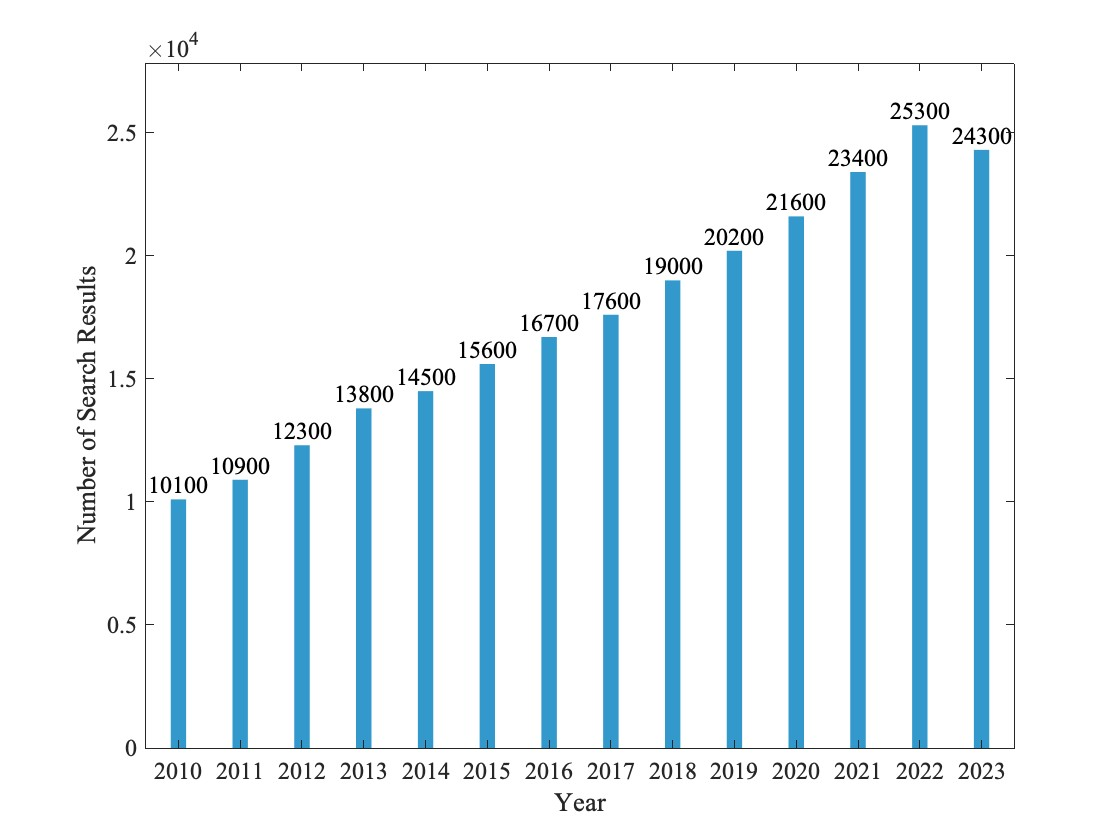
\includegraphics[width=1\textwidth]{00_Images/00_Literature_Review/00_PEMFC_July_12_2024_v1.jpg}  % Change "example-image" to the filename of your image
        \caption{This is an example image.}
        \label{fig:example1}
    \end{figure}

    \begin{figure}[H]
        \centering
        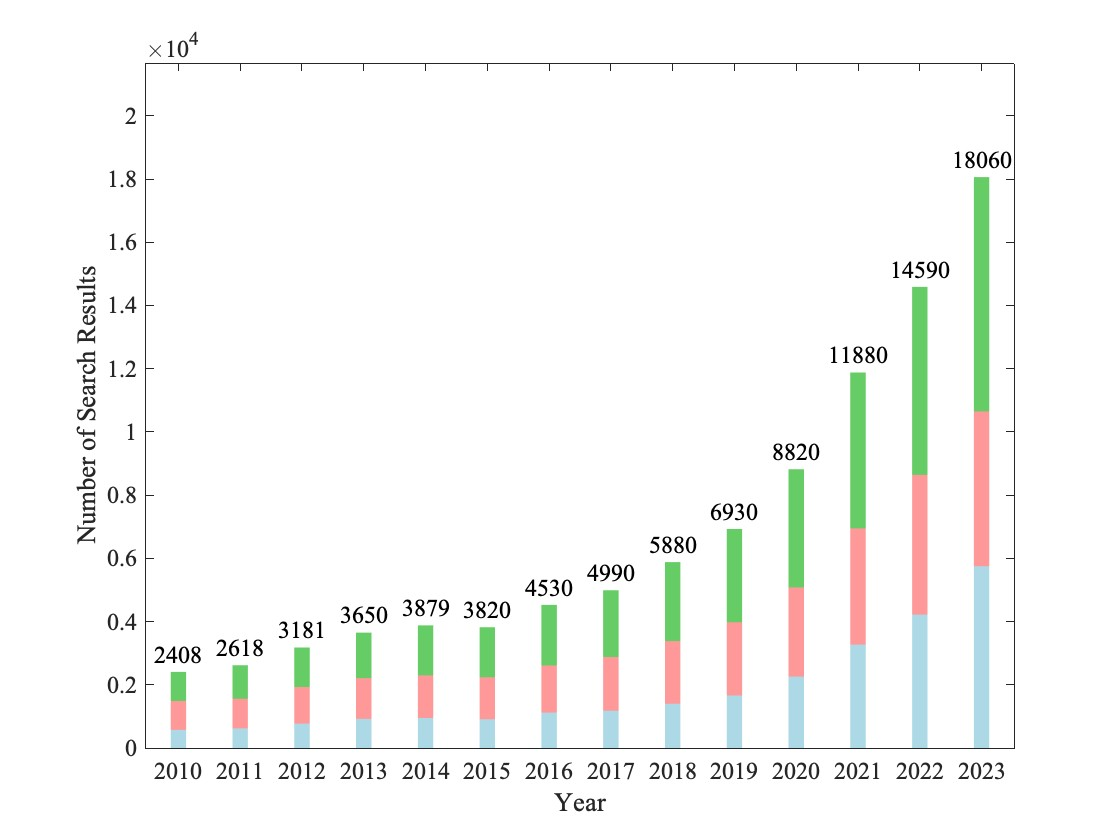
\includegraphics[width=1\textwidth]{00_Images/00_Literature_Review/00_PEMFC_ML_NN_DL_July_12_2024_v1.jpg}  % Change "example-image" to the filename of your image
        \caption{This is an example image.}
        \label{fig:example1}
    \end{figure}

\section{Relevant literature}

    Since the previous work of Yong Rui Than provides a comprehensive overview of the literature on PEMFC involving machine learning. 
    \noindent My review focused on the literature that was not covered in the previous work (i.e. 2021 - 2024). This will ensure that the literature review is up-to-date and relevant to the current state of the field.
    
    \newpage \begin{table}[H]
    \centering
    \begin{tabularx}{\textwidth}{HIJ} % Custom column widths
    \toprule
    \textbf{Title} & \textbf{Author} & \textbf{Summary} \\ 
    \midrule
    Deep learning from three-dimensional multiphysics simulation in operational optimization and control of polymer electrolyte membrane fuel cell for maximum power & Tian et al. & This study integrates an artificial neural network (ANN) with a genetic algorithm (GA) to optimize the operational control of polymer electrolyte membrane fuel cells (PEMFCs) for maximum power output. Utilizing a 3D multiphysics model, 1500 data points were generated to train the ANN, which identified a peak power density of 0.78 W/cm² at 368.8 K. The ANN-GA method effectively predicted performance and optimized conditions across temperatures from 323 K to 373 K, proving crucial for practical system design and rapid control. \\
    \midrule
    Predicting optimal membrane hydration and ohmic losses in operating fuel cells with machine learning & Paciocco et al. & This study pioneers the use of machine learning to predict optimal membrane hydration in polymer electrolyte membrane (PEM) fuel cells, focusing on high frequency resistance (HFR) and optimal hydration current density (OHCD). The long short-term memory recurrent neural network model achieved a mean absolute percentage error of 3.11\% and an R² of over 0.95 in predicting HFR, while deep learning and k-nearest neighbors models predicted OHCD with over 98\% precision and recall. These models provide robust tools for real-time parameter estimation and control, enhancing the performance and reliability of PEM fuel cells and other electrochemical devices. \\
    \midrule
    Pre-diagnosis of flooding and drying in proton exchange membrane fuel cells by bagging ensemble deep learning models using long short-term memory and convolutional neural networks & Kim et al. & This study develops a pre-diagnosis system for detecting flooding and drying in polymer electrolyte membrane fuel cells (PEMFCs) using deep learning models. The system employs long short-term memory (LSTM) and convolutional neural networks (CNN) reinforced by a bagging ensemble method, achieving detection rates of 98.52\% for flooding and 95.36\% for drying within a 30-second prediction window. Experimental data from full-scale single-cell tests, including output voltage, relative humidity, and cell temperature, were used to train the model, highlighting its potential for enhancing PEMFC stability through early fault detection. \\
    \midrule
    Machine learning modeling for proton exchange membrane fuel cell performance & Legala et al. & This study utilizes various machine learning techniques, including Artificial Neural Networks (ANN) and Support Vector Machine Regressor (SVR), to model proton exchange membrane fuel cell (PEMFC) performance and internal states. The ANN model, incorporating the dropout technique, achieved an \(R^2 \geq 0.99\) for predicting cell voltage, membrane resistance, and hydration level across different operating conditions, outperforming SVR in multivariable regression tasks. The models were developed using data from a physics-based semi-empirical model and a 1-D reduced-dimension Computational Fluid Dynamics model, demonstrating that advanced machine learning can create accurate predictive models without extensive physical experimentation. \\
    \midrule 
    \multicolumn{3}{c}{The table continues on the next page...} \\
    \bottomrule
    \end{tabularx}
    \end{table}

    \newpage \begin{table}[H]
    \centering
    \begin{tabularx}{\textwidth}{HIJ} % Custom column widths
    \toprule
    \textbf{Title} & \textbf{Author} & \textbf{Summary} \\ 
    \midrule
    Analysis and modeling of high-performance polymer electrolyte membrane electrolyzers by machine learning & Gunay et al. & This study employs box and whisker plots, principal component analysis (PCA), and classification and regression tree modeling to analyze and model high-performance polymer electrolyte membrane (PEM) electrolyzers using a database of 789 data points from 30 recent publications. The PCA identified performance risks associated with specific materials, such as cathode surfaces with high Ni content and anode surfaces with cobalt-iron alloys or RuO2. Classification trees highlighted current density, potential, and mole fractions of Ni and Co as key performance variables, while the regression tree technique accurately modeled polarization behavior with an RMSE of 0.18. \\
    \midrule 
    Machine learning optimization of operating parameters to achieve high power density and efficiency of polymer electrolyte membrane fuel cell & Kaiser et al. & This study employs five machine learning regression models—Artificial Neural Network (ANN), Decision Tree (DT), Random Forest (RF), Gradient Boosting (GB), and Extreme Gradient Boosting (xGB)—to optimize the operating parameters of polymer electrolyte membrane fuel cells (PEMFCs) for maximum power density and efficiency. Among these models, the GB regressor demonstrated the highest accuracy with an \(R^2 = 0.973\) and an \(MSE = 0.0088\) for testing data, excelling in replicating experimental polarization curves. The optimal operating conditions identified were anode and cathode pressures at 2 bar and cathode stoichiometry between 2.50–2.75, significantly enhancing PEMFC performance. The study highlights the GB model's superior capability in handling extensive datasets and optimizing complex nonlinear operational conditions, thus offering a novel approach for PEMFC performance optimization. \\
    \midrule
    A Review of physics-based and data-driven models for real-time control of polymer electrolyte membrane fuel cells & Zhao et al. & This review critically examines recent advancements in physics-based and data-driven models for the real-time control of polymer electrolyte membrane (PEM) fuel cells. Emphasizing the need for models that balance accuracy and computational efficiency, the study highlights trends such as coupling single cell models with balance-of-plant systems, incorporating aging effects for long-term predictions, and leveraging artificial intelligence algorithms for enhanced computational speed. Among the models reviewed, the study notes the superior accuracy and speed of data-driven models, particularly when trained on extensive datasets, while also addressing challenges in their applicability across diverse operational conditions. \\
    \midrule
    Application of Machine Learning in Optimizing Proton Exchange Membrane Fuel Cells: A Review & Ding et al. & This review explores the application of machine learning (ML) in optimizing proton exchange membrane fuel cells (PEMFCs) to address their cost and performance challenges for large-scale commercialization. The study highlights ML's capability to reduce experimental and computational costs by predicting outcomes based on datasets from experiments or theoretical simulations. Notable ML applications in this field include predicting active electrocatalysts, optimizing membrane electrode assemblies (MEA), designing efficient flow channels, and developing stack operation strategies. \\
    \midrule
    \multicolumn{3}{c}{The table continues on the next page...} \\
    \bottomrule
    \end{tabularx}
    \end{table}

    \newpage \begin{table}[H]
    \centering
    \begin{tabularx}{\textwidth}{HIJ} % Custom column widths
    \toprule
    \textbf{Title} & \textbf{Author} & \textbf{Summary} \\ 
    \midrule
    Towards Reliable Prediction of Performance for Polymer Electrolyte Membrane Fuel Cells via Machine Learning-Integrated Hybrid Numerical Simulations & Kaiser et al. & This study explores hybrid numerical simulations integrating machine learning (ML) to enhance the reliability and accuracy of polymer electrolyte membrane fuel cell (PEMFC) performance predictions. By addressing the limitations of existing computational fluid dynamics (CFD) models, which suffer from simplifications and inaccurate parameter approximations, the study demonstrates how ML can provide more appropriate parameters, leading to improved electrochemistry, mass/species transfer, thermal management, and water transport modeling. The ML-assisted CFD models are shown to optimize component design and material properties, significantly enhancing PEMFC efficiency and providing a robust framework for future PEMFC development and its impact on the transportation sector. \\
    \midrule
    An Optimized Data Analysis on a Real-Time Application of PEM Fuel Cell Design by Using Machine Learning Algorithms & Saco et al. & This study applies machine learning algorithms to optimize the design of polymer electrolyte membrane fuel cells (PEMFCs) by analyzing their performance under different humidity levels. Three machine learning models—Support Vector Machine Regressor (SVMR), Linear Regression (LR), and k-Nearest Neighbors (KNN)—were evaluated for their predictive accuracy using root mean square error (RMSE) as the metric. The LR model demonstrated superior performance with an RMSE of 0.0034, compared to 0.0046 for SVMR and 0.004 for KNN, effectively enhancing PEMFC efficiency through optimal humidification conditions. \\
    \midrule
    A systematic review of machine learning methods applied to fuel cells in performance evaluation, durability prediction, and application monitoring & Ming et al. & This systematic review explores the application of machine learning (ML) methods, including traditional ML and deep learning (DL), to fuel cells for performance evaluation, durability prediction, and application monitoring. The review highlights ML's effectiveness in addressing complex phenomena such as mass/heat transfer and electrochemical reactions, crucial for improving energy efficiency and durability. Notably, ML models excel in material selection, chemical reaction modeling, polarization curves, state of health monitoring, fault diagnostics, and predicting remaining useful life. The study also compares ML and DL methods, and their integration with physics simulations, providing a comprehensive outlook on future research directions for ML applications in fuel cells. \\
    \midrule
    Application of Machine Learning in Fuel Cell Research & Su et al. & This comprehensive review examines the application of machine learning (ML) algorithms in optimizing proton exchange membrane fuel cells (PEMFCs), focusing on performance prediction, service life estimation, and fault diagnosis. The study highlights the effectiveness of ML models, such as artificial neural networks (ANN), support vector machines (SVM), and random forests (RF), in solving nonlinear problems associated with PEMFCs. Notable findings include an RMSE of 0.0034 for linear regression in performance prediction, a 99\% accuracy rate in power-current curve modeling using SVM, and high precision in fault diagnosis and service life prediction. \\
    \midrule
    \multicolumn{3}{c}{The table continues on the next page...} \\
    \bottomrule
    \end{tabularx}
    \end{table}

    \newpage \begin{table}[H]
    \centering
    \begin{tabularx}{\textwidth}{HIJ} % Custom column widths
    \toprule
    \textbf{Title} & \textbf{Author} & \textbf{Summary} \\ 
    \midrule 
    Optimization of Proton Exchange Membrane Electrolyzer Cell Design Using Machine Learning & Mohamed et al. & This study leverages machine learning (ML) models, specifically polynomial and logistic regression, to optimize the design of proton exchange membrane (PEM) electrolyzer cells. By predicting eleven parameters of cell components based on four input parameters (hydrogen production rate, cathode area, anode area, and cell design type), the models achieved an average accuracy of 83.6\% and a mean absolute error (MAE) of 6.825. Validated on a test set, the ML models demonstrated excellent agreement with experimental results, showing a negligible MAE of 0.615 in hydrogen production rate predictions. The study successfully designed optimal PEM electrolyzer cells for commercial-scale hydrogen production rates (500 to 5000 mL/min), highlighting the potential of ML to significantly reduce the cost and time required for developing efficient water electrolyzers. \\
    \bottomrule
    \end{tabularx}
    \caption{Database review of literature on PEMFC and machine learning from 2021 to 2024}
    \end{table}

\chapter{Materials and Methods}
\newpage \begin{table}[H]
\centering
\begin{tabularx}{\textwidth}{DEFG} % Custom column widths
\toprule
\textbf{Header} & \textbf{Symbol} & \textbf{Explanation} & \textbf{Unit} \\ 
\midrule
\multicolumn{4}{c}{\textbf{Input Parameters}} \\
\midrule
Q & \( Q \) & \textbf{Heat generation} influences membrane hydration and operational efficiency; critical to prevent membrane dry-out and maintain ion conductivity. & \( \text{Wm}^{-2} \) \\
Tamb & \( T_{amb} \) & \textbf{Ambient temperature of the air} sets baseline thermal conditions; higher temperatures boost performance to a limit before causing potential overheating. & \( \degree C \) \\
Uin & \( U_{in} \) & \textbf{Airflow velocity} determines oxygen supply rate, essential for maintaining optimal reaction rates and power output. & \( \text{m/s} \) \\
Wcc & \( W_{cc} \) & \textbf{Cathode channel width} determines oxygen flow and diffusion rates to the cathode, crucial for optimizing reaction efficiency. & \( \text{mm} \) \\
Hcc & \( H_{cc} \) & \textbf{Cathode channel height} affects gas flow resistance and water removal, essential for maintaining membrane hydration and preventing flooding. & \( \text{mm} \) \\
Lcc & \( L_{cc} \) & \textbf{Cathode channel length} influences the residence time of reactants and products along the channel, impacting overall fuel cell efficiency. & \( \text{mm} \) \\ 
Wr & \( W_{r} \) & \textbf{Rib width} supports mechanical stability and maximizes the active area available for reactions, balancing structural support with performance. & \( \text{mm} \) \\
Hr & \( H_{r} \) & \textbf{Rib height} controls the depth of flow channels, enhancing reactant distribution and efficient water management within the stack. & \( \text{mm} \) \\
\midrule
\multicolumn{4}{c}{\textbf{Output Performance Metrics}} \\
\midrule
Tsta & \( T_{stack} \) & \textbf{Stack temperature} is crucial for optimal reaction rates, membrane hydration, and to prolong the lifespan. & \( \degree C \) \\ 
Delp & \( \Delta p \) & \textbf{Pressure drop} indicates the system's resistance to reactant flow; minimizing pressure drop is essential to enhance efficiency and ensure uniform distribution. & \( \text{Pa} \) \\ 
\bottomrule
\end{tabularx}
\caption{Detailed Explanation of Variables}
\end{table}
    
\chapter{COMSOL Model}
\section{Model Assumptions}
    \begin{enumerate}
        \item The airflow entering the channel is turbulent. The Reynolds number exceeds 2300 at an inlet velocity ($U_{in}$) of 0.3 m/s.
        \item Portions of the fuel cell not part of the cathode flow field are impermeable to air. While carbon paper is porous, the in-plane pressure drop is much greater than that of the cathode flow field.
        \item The cathode flow field channels are modeled with a uniform height. The average offset (0.025 mm) is negligible compared to the channel height (1 mm).
        \item Cathode flow fields are modeled with straight edges and right-angle folds. The fold radius (0.05 mm) is small compared to the channel width (1 mm).
        \item Conservation of mass and momentum of airflow is assumed to be valid when transitioning between open spaces and cathode channels.
        \item A representative unit cell approximates the entire stack, excluding edge effects near the terminals. Airflow entering the unit cell is uniform and symmetrical.
        \item Channels are identical throughout the stack, resulting in no pressure drop differences between channels.
        \item The channels are fully dry without condensation. The oxidant stoichiometry exceeds 100, ensuring water vapor produced is absorbed by the airflow, negating the need for accounting water saturation.
        \item The losses from the fuel cell operation are converted to heat. 
    \end{enumerate}

    \section{Workflow - Pressure Drop}
    The following steps outline the workflow process for the unit cell simulations conducted in COMSOL:

    \begin{enumerate}
        \item \textbf{Selection of Laminar Flow Model:}
        \begin{itemize}
            \item This model was chosen because the airflow within the channels is laminar and is the largest contributor to the pressure drop across the stack.
            \item The laminar flow model allows for faster convergence and has been shown to be accurate when compared with experimental results.
        \end{itemize}
        
        \item \textbf{Construction of Unit Cell:}
        \begin{itemize}
            \item The unit cell was constructed using blocks with dimensions defined by equations to accommodate dimensional changes in the channels.
        \end{itemize}
        
        \item \textbf{Meshing Strategy:}
        \begin{itemize}
            \item A custom mesh was employed, focusing on the transition areas between inflow and outflow within the channels with a finer mesh.
            \item A coarser mesh was used within the channel and the air space between inflow and outflow.
            \item A mesh independence study was performed during the mesh fine-tuning. The results are shown in Figure ?.
            \item The difference between the blue dash (custom meshing) and green dots (physics-based extra fine meshing) is less than 3\%, thus the blue dash mesh was selected for its speed and accuracy.
        \end{itemize}
        
        \item \textbf{Parameter Sweep Function:}
        \begin{itemize}
            \item The parameter sweep function was utilized to explore all possible combinations for each stack size.
        \end{itemize}
        
        \item \textbf{Exporting Simulation Data:}
        \begin{itemize}
            \item The inputs and outputs of the simulations were exported from COMSOL for further analysis.
        \end{itemize}
    \end{enumerate}

    \section{Workflow - Temperature Stack}
    The following steps outline the workflow process for the unit cell simulations conducted in COMSOL:

    \begin{enumerate}
        \item \textbf{Selection of Physics Models:}
        \begin{itemize}
            \item The unit cell simulations were done using laminar flow physics as well as heat transfer in laminar flow.
            \item The parameter sweep function was utilized to explore all possible combinations in the parameter space.
            \item This model was selected because the flow through the channel is laminar and the simulation focuses on heat transfer within the channels.
        \end{itemize}
        
        \item \textbf{Construction of Unit Cell:}
        \begin{itemize}
            \item The unit cell was constructed using blocks with dimensions defined by equations to accommodate dimensional changes in the channels.
        \end{itemize}
        
        \item \textbf{Heat Generation Simulation:}
        \begin{itemize}
            \item Heat generation was simulated as a boundary heat source placed at the cathode side of the membrane.
        \end{itemize}
        
        \item \textbf{Heat Conduction Values:}
        \begin{itemize}
            \item The heat conduction values for each layer in the fuel cell were obtained from various papers, as shown in Table 8-1.
        \end{itemize}
        
        \item \textbf{Meshing Strategy:}
        \begin{itemize}
            \item A mesh independence study was conducted during the fine-tuning of the mesh. The results are shown in Figure ?.
            \item The difference between the blue dash and green dots is less than 1.06\%, hence the blue dash mesh was selected for its speed and accuracy.
        \end{itemize}
        
        \item \textbf{Exporting Simulation Data:}
        \begin{itemize}
            \item The inputs and outputs of the simulations were exported from COMSOL for further analysis.
        \end{itemize}
    \end{enumerate}

\newpage \section{Parameters}

    \begin{table}[h]
    \centering
    \begin{tabularx}{\textwidth}{X X X}
    \toprule
    \textbf{Name} & \textbf{Value} & \textbf{Unit} \\ 
    \midrule
    Cell Area & 0.005 & m$^2$ \\ 
    Cell Voltage & 0.6 & V \\ 
    Compression & 0.1 & - \\ 
    Current & 40 & A \\ 
    Hbp & 5$\times$10$^{-5}$ & m \\ 
    Hcc & 1.25$\times$10$^{-3}$ & m \\ 
    Hcp & 3.15$\times$10$^{-4}$ & m \\ 
    Hmem & 1.5$\times$10$^{-5}$ & m \\ 
    Kcp & 1.5 & W$\cdot$m$^{-1}$K$^{-1}$ \\ 
    Kmem & 0.1 & W$\cdot$m$^{-1}$K$^{-1}$ \\ 
    Lcc & 0.03 & m \\ 
    pRef & 1.0133$\times$10$^5$ & Pa \\ 
    Q & 5040 & W$\cdot$m$^{-2}$ \\ 
    Tamb & 293.15 & K \\ 
    Test & 25.2 & W \\ 
    Uin & 7.75 & m$\cdot$s$^{-1}$ \\ 
    Wcc & 0.001 & m \\ 
    Wr & 5$\times$10$^{-5}$ & m \\ 
    \bottomrule
    \end{tabularx}
    \caption{Parameter Values}
    \label{tab:parameters}
    \end{table}

\section{Materials}
    % Superscripts Table
    \begin{table}[H]
    \centering
    \begin{tabularx}{\textwidth}{BA}
    \toprule
    \textbf{Name} & \textbf{Unit} \\ 
    \midrule
    \multicolumn{2}{c}{\textbf{Air}} \\
    \midrule
    Dynamic viscosity & \( \text{Pa} \cdot \text{s} \) \\ 
    Ratio of specific heats & - \\ 
    Heat capacity at constant pressure & \(\text{J} / (\text{kg} \cdot \text{K})\) \\ 
    Density & \(\text{kg} / \text{m}^{3}\) \\ 
    Thermal conductivity & \(\text{W} / (\text{m} \cdot \text{K})\) \\
    \midrule
    \multicolumn{2}{c}{\textbf{Carbon Paper}} \\
    Density & \(\text{kg} / \text{m}^{3}\) \\ % No value
    Heat capacity at constant pressure & \(\text{J} / (\text{kg} \cdot \text{K})\) \\ % No value
    Thermal conductivity & \(\text{W} / (\text{m} \cdot \text{K})\) \\
    \midrule
    \midrule
    \multicolumn{2}{c}{\textbf{Membrane}} \\
    Thermal conductivity & \(\text{W} / (\text{m} \cdot \text{K})\) \\
    \midrule
    \midrule
    \multicolumn{2}{c}{\textbf{Steel Grade 316L}} \\
    Density & \(\text{kg} / \text{m}^{3}\) \\ % No value
    Heat capacity at constant pressure & \(\text{J} / (\text{kg} \cdot \text{K})\) \\ % No value
    Thermal conductivity & \(\text{W} / (\text{m} \cdot \text{K})\) \\
    \midrule
    \bottomrule
    \end{tabularx}
    \caption{Material Descriptions}
    \end{table}


\section{Laminar Flow}
    \subsection{Governing Equations}
        \begin{equation}
            \rho (\textbf{u} \cdot \nabla) \textbf{u} = \nabla \cdot \left[-p\textbf{I} + \textbf{K} \right] + \textbf{F} 
        \end{equation}
            \noindent where \(\rho\) is the density of air, \textbf{u} is the velocity vector, p is the pressure, \textbf{I} is the identity matrix, \textbf{K} is the viscous stress tensor, and \textbf{F} is the volume force vector.
        \begin{equation}
            \nabla \cdot (\rho \textbf{u})= 0 % The equation is different in the thesis
        \end{equation}
        \begin{equation}
            \textbf{K} = \mu (\nabla \textbf{u} + (\nabla \textbf{u})^T) - \frac{2}{3} \mu (\nabla \cdot \textbf{u})\textbf{I} % NOTE: The equation is different from the one in the thesis.
        \end{equation}
            where \textbf{\(\mu\)} is the dynamic viscosity of air. 

    \subsection{Initial Values}
        \begin{enumerate}
            \item Velocity field
                \begin{equation}
                    \textbf{u} = \textbf{0}
                \end{equation}
            \item Pressure
                \begin{equation}
                    p = 0
                \end{equation}
        \end{enumerate}

    \subsection{Boundary Conditions}
        \begin{enumerate}
            \item Wall (No slip)
                \begin{equation}
                    \mathbf{u} = \mathbf{0}
                \end{equation}
        
            \item Inlet (Velocity)
                \begin{equation}
                    \mathbf{u} = -U_{0} \mathbf{n}
                \end{equation}
                    where \(U_{0}\) is the initial velocity (i.e. normal inflow velocity) and \(\mathbf{n}\) is the unit normal vector. 
            
            \item Outlet (Pressure)
                \begin{equation}
                    \left[-p\textbf{I} + \textbf{K} \right]\mathbf{n} = - \hat{p}_{0} \mathbf{n} % this equation is different from the one in the thesis.
                \end{equation}
                \begin{equation}
                    \hat{p_{0}} \leq p_{0}, \nabla \mathbf{G} \cdot \mathbf{n} = 0
                \end{equation}
                    where \(\hat{p}_{0}\) is the estimated standard condition pressure, \(p_{0}=0\) is the standard condition pressure (i.e. suppress backflow), \(\mathbf{G}\) is the reciprocal wall distance. 
        
            \item Symmetry 
                \begin{equation}
                    \mathbf{u} \cdot \mathbf{n} = 0
                \end{equation}
                \begin{equation}
                    \mathbf{K}_{n} - (\mathbf{K}_{n} \cdot \mathbf{n})\mathbf{n} = 0, \mathbf{K}_{n} = \mathbf{Kn}
                \end{equation}
        \end{enumerate}
        
\section{Heat Transfer}
    \subsection{Governing Equations - Solid}
        \begin{equation}
            \rho C_{p} \textbf{u} \cdot \nabla T + \nabla \cdot \textbf{q} = Q + Q_{ted}
        \end{equation}
            \noindent where \(C_{p}\) is the specific heat capacity of air, T is the temperature of air, \textbf{q} is the heat flux vector, Q is the heat source, and \(Q_{ted}\) is the thermoelastic damping heat source.
        \begin{equation}
            \textbf{q} = -k \nabla T
        \end{equation}
            \noindent where k is the thermal conductivity. 
        \begin{equation}
            Q = (1.23 - Operating\ Voltage) \times \frac{Fuel\ Cell\ Stack\ Current}{Cell\ Area}
        \end{equation}
            
    \subsection{Governing Equations - Fluid}
        \begin{equation}
            \rho C_{p} \textbf{u} \cdot \nabla T + \nabla \cdot \textbf{q} = Q + Q_{p} + Q_{vd} % I dont know what vd is.
        \end{equation}
        \noindent where \(Q_{p}\) is the point heat source.
        \begin{equation}
            \textbf{q} = -k \nabla T
        \end{equation}
    
    \subsection{Governing Equations - Thin Layer}
        \begin{equation}
            -\textbf{n}_{d} \cdot \textbf{q}_{u} = \frac{(T_{u} - T_{d})}{R_{s}} + \frac{1}{2} d_{s} Q_{s}
        \end{equation}
        \noindent where \(R_s\) is the thermal resistance, and \(d_s\) is the thin layer thickness. 
        \begin{equation}
            -\textbf{n}_{u} \cdot \textbf{q}_{u} = \frac{(T_{d} - T_{u})}{R_{s}} + \frac{1}{2} d_{s} Q_{s}
        \end{equation}
        \begin{equation}
            R_{s} = \frac{d_{s}}{k_{s}}
        \end{equation}
    
    \subsection{Initial Values}
        \begin{enumerate}
            \item Temperature
                \begin{equation}
                    T = T_{amb}
                \end{equation}
                where \(T_{amb}\) is the initial ambient temperature.
        \end{enumerate}

    \subsection{Boundary Conditions}
        \begin{enumerate}
            \item Insulation
                \begin{equation}
                    -\mathbf{n} \cdot \mathbf{q} = 0
                \end{equation}
        
            \item Symmetry
                \begin{equation}
                    -\mathbf{n} \cdot \mathbf{q} = 0
                \end{equation}
        
            \item Boundary Heat Source
                \begin{equation}
                    -\mathbf{n} \cdot \mathbf{q} = Q_b
                \end{equation}
                where \(Q_b\) is the boundary heat source.
            
            \item Outflow
                \begin{equation}
                    -\mathbf{n} \cdot \mathbf{q} = 0
                \end{equation}
        
            \item Inlet
                \begin{equation}
                    T = T_{amb}
                \end{equation}
        \end{enumerate}

\section{Mesh}

\section{Study}
    \subsection{Difference between External and Internal Sweep}
        An internal sweep involves varying parameters directly within the 
        simulation model itself. This type of sweep is integrated into the 
        simulation process, where the solver automatically adjusts the parameters 
        as part of its internal algorithm. Internal sweeps are typically used to 
        explore the parameter space of the model in a more automated and 
        controlled manner, often leveraging the solver's built-in capabilities 
        to iterate through different parameter values.

        
        \vspace{1em} \noindent An external sweep, on the other hand, involves varying parameters outside 
        of the simulation model. This is usually managed by an external script 
        or control mechanism that systematically modifies the input parameters, 
        runs the simulation for each set of parameters, and collects the results. 
        External sweeps provide more flexibility and control over the parameter 
        variations and can be useful for complex scenarios where the internal 
        capabilities of the solver might be limited.
    \subsection{Parametric Sweep}
        A parametric sweep is a systematic method used in simulations and computational 
        experiments to explore the effects of varying parameters within a defined range. 
        By adjusting one or more input parameters incrementally, researchers can observe 
        how changes influence the outcome, enabling a comprehensive analysis of the 
        system's behavior. This technique is essential for optimizing designs, 
        identifying critical factors, and understanding the sensitivity of the results 
        to different variables. Ultimately, parametric sweeps provide valuable insights 
        that drive informed decision-making and innovation.

        \begin{table}[h]
        \centering
        \begin{tabularx}{\textwidth}{X X X}
        \toprule
        \textbf{Name} & \textbf{Values} & \textbf{Unit} \\ 
        \midrule
        Hcc & 1 1.25 1.5 1.75 2 & \(\text{mm}\) \\ 
        Wcc & 0.5 0.75 1 1.25 1.5 & \(\text{mm}\) \\ 
        Lcc & 30 60 90 & \(\text{mm}\) \\ 
        \bottomrule
        \end{tabularx}
        \caption{Parameter Sweep Values for All Combinations}
        \end{table}
    \subsection{Auxilary Sweep}
        An auxiliary sweep is a computational technique used to study the influence
        of secondary parameters or variables that are not directly part of the main 
        parametric study. It involves varying these auxiliary parameters to 
        investigate their impact on the primary simulation or experiment results. 
        This approach helps in understanding the interactions and dependencies 
        between primary and auxiliary parameters, providing a deeper insight into 
        the system's overall behavior. Auxiliary sweeps are particularly useful in 
        complex models where multiple factors may indirectly affect the outcomes, 
        aiding in fine-tuning and enhancing the accuracy of simulations.

        \begin{table}[h]
        \centering
        \begin{tabularx}{\textwidth}{X X X}
        \toprule
        \textbf{Name} & \textbf{Values} & \textbf{Unit} \\ 
        \midrule
        Uin & 1 3.25 5.5 7.75 10 & \(\text{m}/\text{s}\) \\ 
        Q & 1272 3132 5040 & \(W/\text{m}^{-2}\) \\ 
        Tamb & -20 0 20 40 & \(\degree \text{C}\) \\ 
        \bottomrule
        \end{tabularx}
        \caption{Auxilary Sweep Values for All Combinations}
        \end{table}
    
    \section{Results}
        \subsection{Accumulated Probe Table: Set 1}
            \begin{enumerate}
                \item Hcc (1 - hc)
                \item Wcc (2 - wc)
                \item Lcc (3 - length)
                \item Tamb (4 - Tamb)
                \item Q (5 - Q)
                \item Uin (6 - Uin)
                \item Delp (15 - Pressure (Pa), Pressure Probe 3)
                    \begin{figure}[H]
                        \centering
                        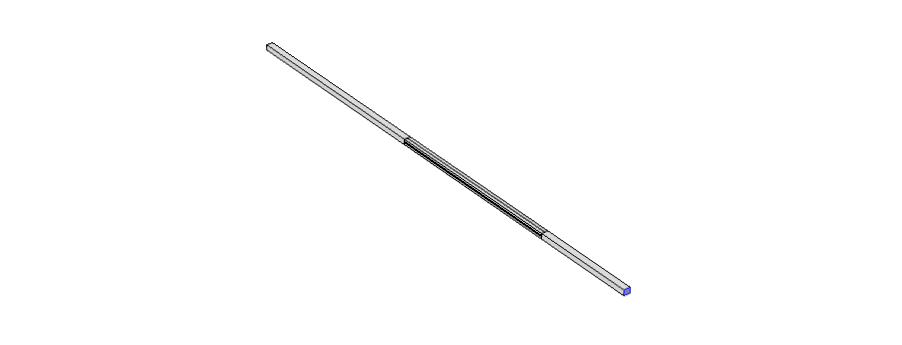
\includegraphics[width=1\textwidth]{00_Images/00_Pressure_Probe_3.png}
                        \caption{Pressure Probe 3 Location}
                    \end{figure}
                \item Tsta (18 - Temperature (degC), Stack Temperature Probe 1)
                    \begin{figure}[H]
                        \centering
                        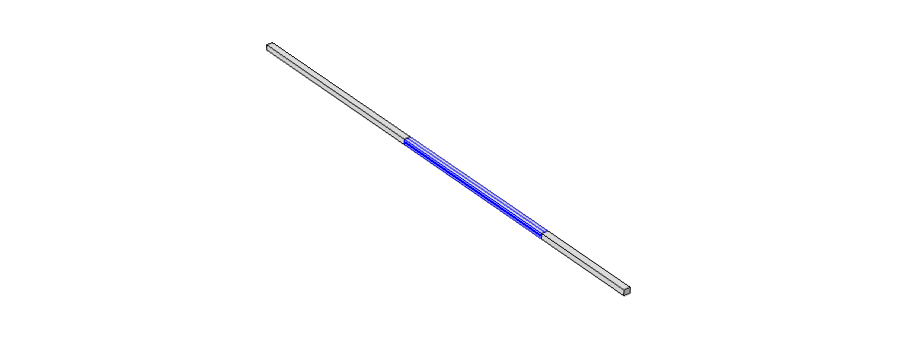
\includegraphics[width=1\textwidth]{00_Images/00_Stack_Temperature_Probe_1.png}
                        \caption{Stack Temperature Probe 1 Location}
                    \end{figure}
            \end{enumerate}

        \subsection{3D Plots}
            \begin{enumerate}
                \item Pressure Drop
                    \begin{figure}[H]
                        \centering
                        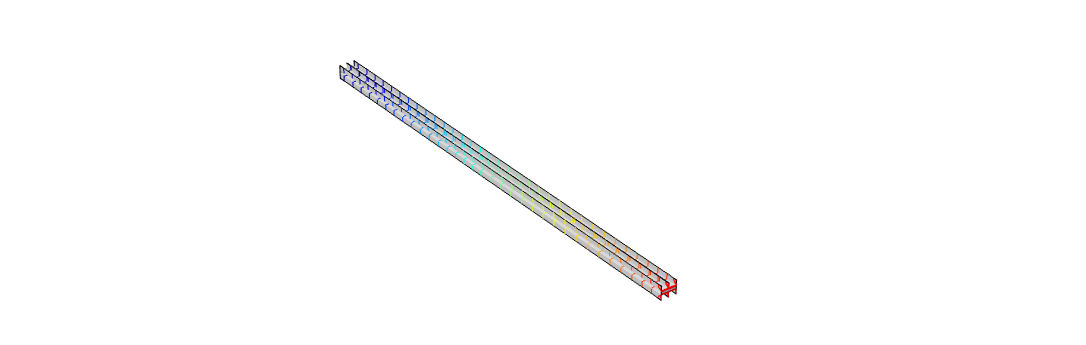
\includegraphics[width=1\textwidth]{00_Images/00_Pressure.png}
                        \caption{Pressure Drop 3D Plot}
                    \end{figure}
                \item Temperature Stack
                    \begin{figure}[H]
                        \centering
                        
\includegraphics[width=1\textwidth]{00_Images/00_Temperature.png}
                        \caption{Temperature Stack 3D Plot}
                    \end{figure}
                \item Velocity 
                    \begin{figure}
                        \centering
                        
\includegraphics[width=1\textwidth]{00_Images/00_Velocity.png}
                        \caption{Velocity 3D Plot}
                    \end{figure}
            \end{enumerate}

\chapter{Dataset \& Data Preprocessing}
\section{Data Preprocessing}
    \subsection{Small Stack}
        \begin{figure}[H]
            \centering
            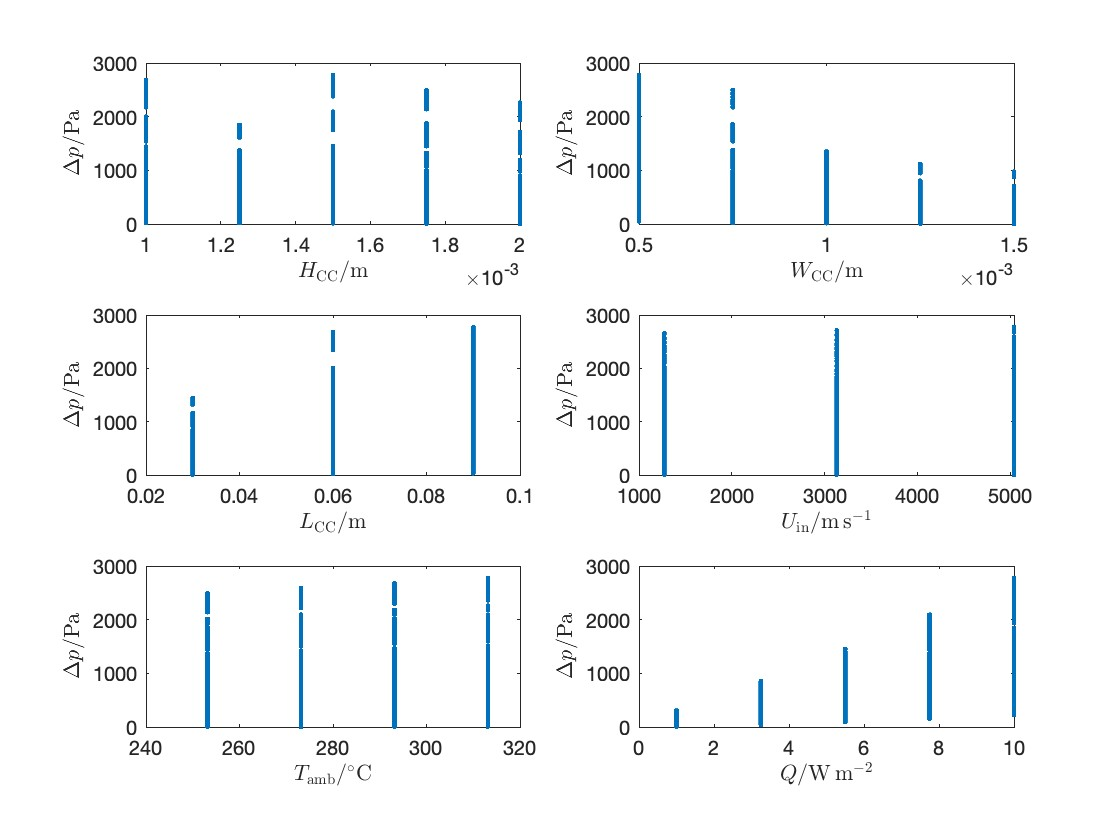
\includegraphics[width=1\textwidth]{00_Images/00_Small_Stack_Images/00_Pressure_Drop_vs_Features_July_10_2024_v1.jpg}  % Change "example-image" to the filename of your image
            \caption{This is an example image.}
            \label{fig:example1}
        \end{figure}

        \begin{figure}[H]
            \centering
            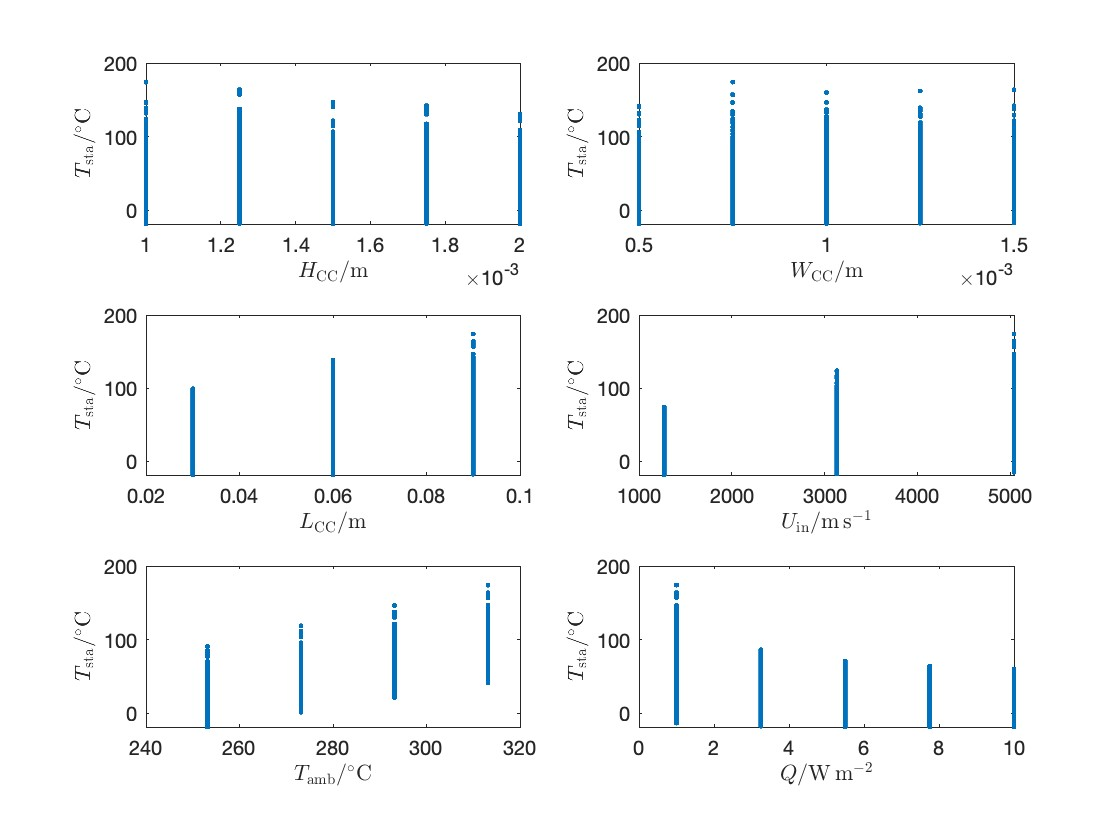
\includegraphics[width=1\textwidth]{00_Images/00_Small_Stack_Images/00_Temperature_vs_Features_July_10_2024_v1.jpg}  % Change "example-image" to the filename of your image
            \caption{This is an example image.}
            \label{fig:example1}
        \end{figure}

        \begin{figure}[H]
            \centering
            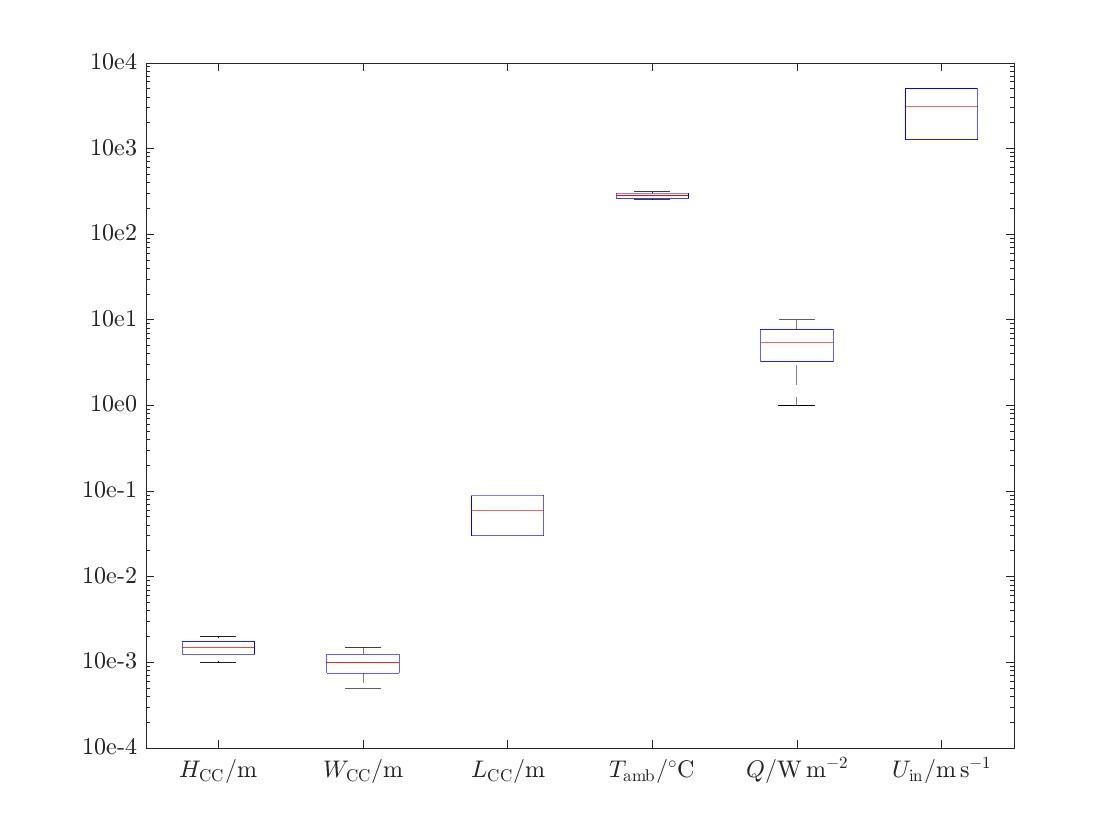
\includegraphics[width=1\textwidth]{00_Images/00_Small_Stack_Images/00_Combined_Boxplot_Features_July_10_2024_v1.jpg}  % Change "example-image" to the filename of your image
            \caption{This is an example image.}
            \label{fig:example1}
        \end{figure}

        \begin{figure}[H]
            \centering
            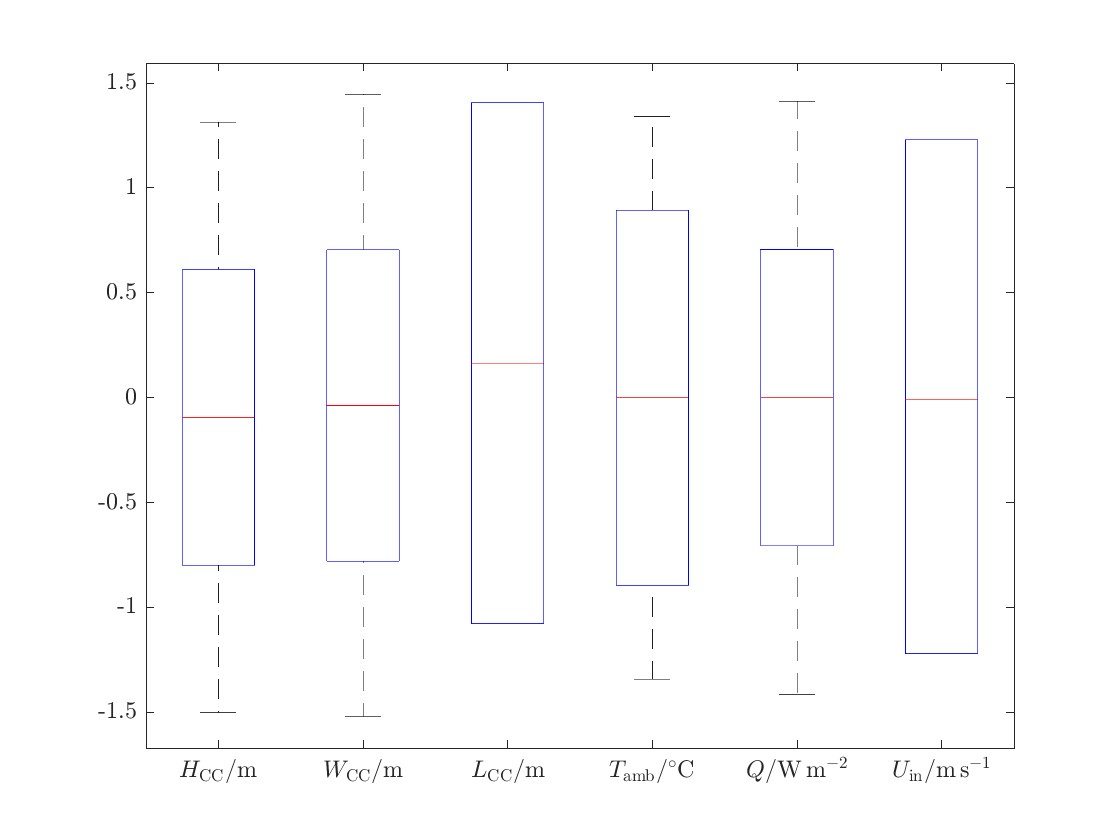
\includegraphics[width=1\textwidth]{00_Images/00_Small_Stack_Images/00_Combined_Boxplot_Normalized_Features_July_10_2024_v1.jpg}  % Change "example-image" to the filename of your image
            \caption{This is an example image.}
            \label{fig:example1}
        \end{figure}

        \begin{figure}[H]
            \centering
            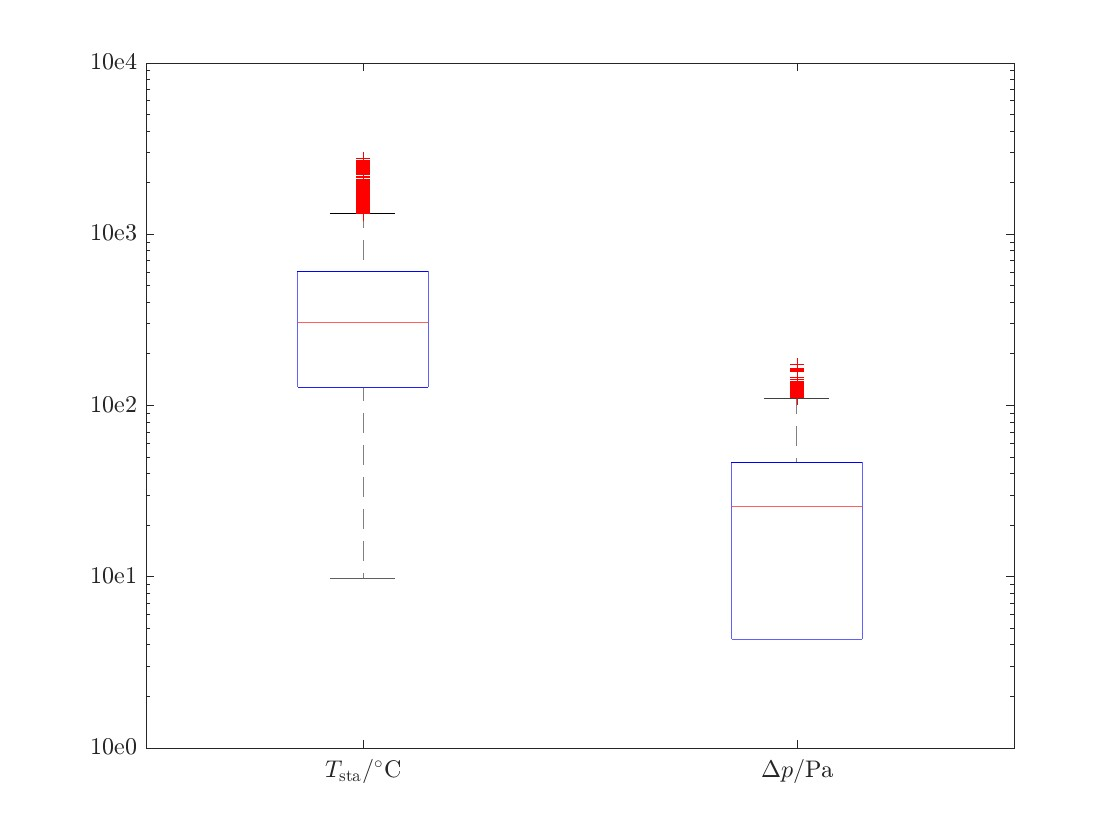
\includegraphics[width=1\textwidth]{00_Images/00_Small_Stack_Images/00_Combined_Boxplot_Outputs_July_10_2024_v1.jpg}  % Change "example-image" to the filename of your image
            \caption{This is an example image.}
            \label{fig:example1}
        \end{figure}

        \begin{figure}[H]
            \centering
            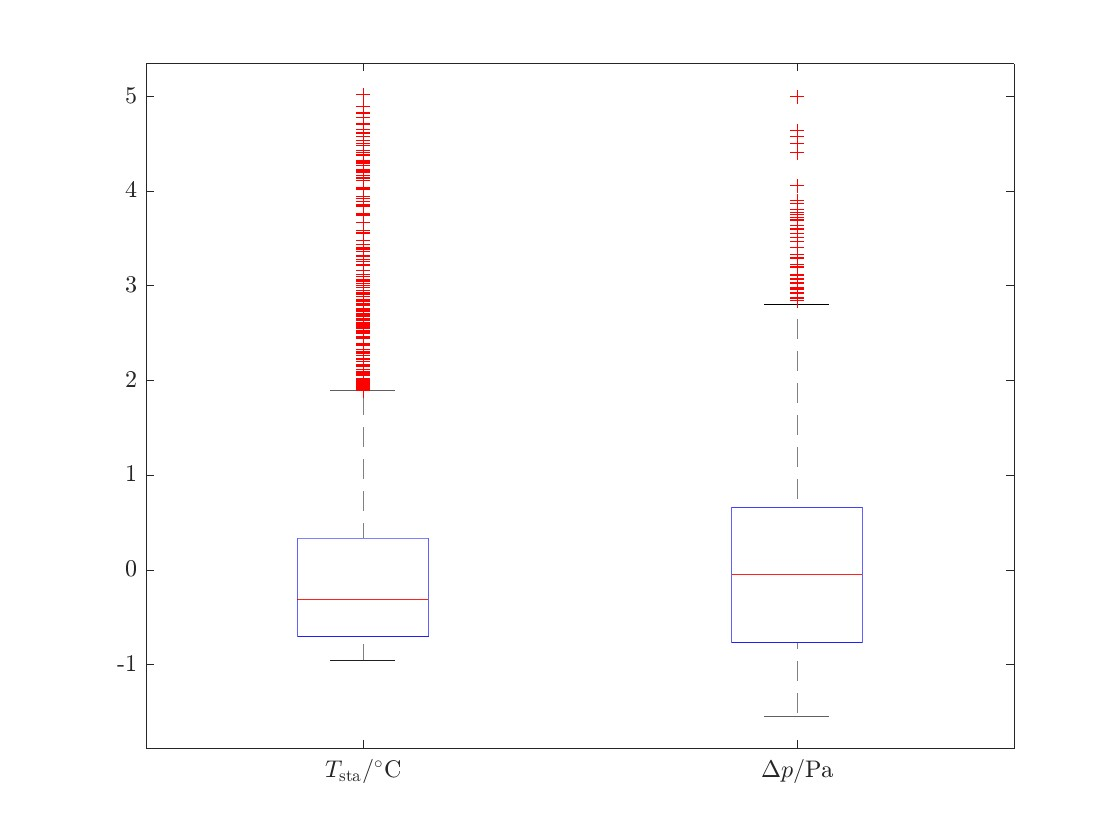
\includegraphics[width=1\textwidth]{00_Images/00_Small_Stack_Images/00_Combined_Boxplot_Normalized_Outputs_July_10_2024_v1.jpg}  % Change "example-image" to the filename of your image
            \caption{This is an example image.}
            \label{fig:example1}
        \end{figure}

        \begin{figure}[H]
            \centering
            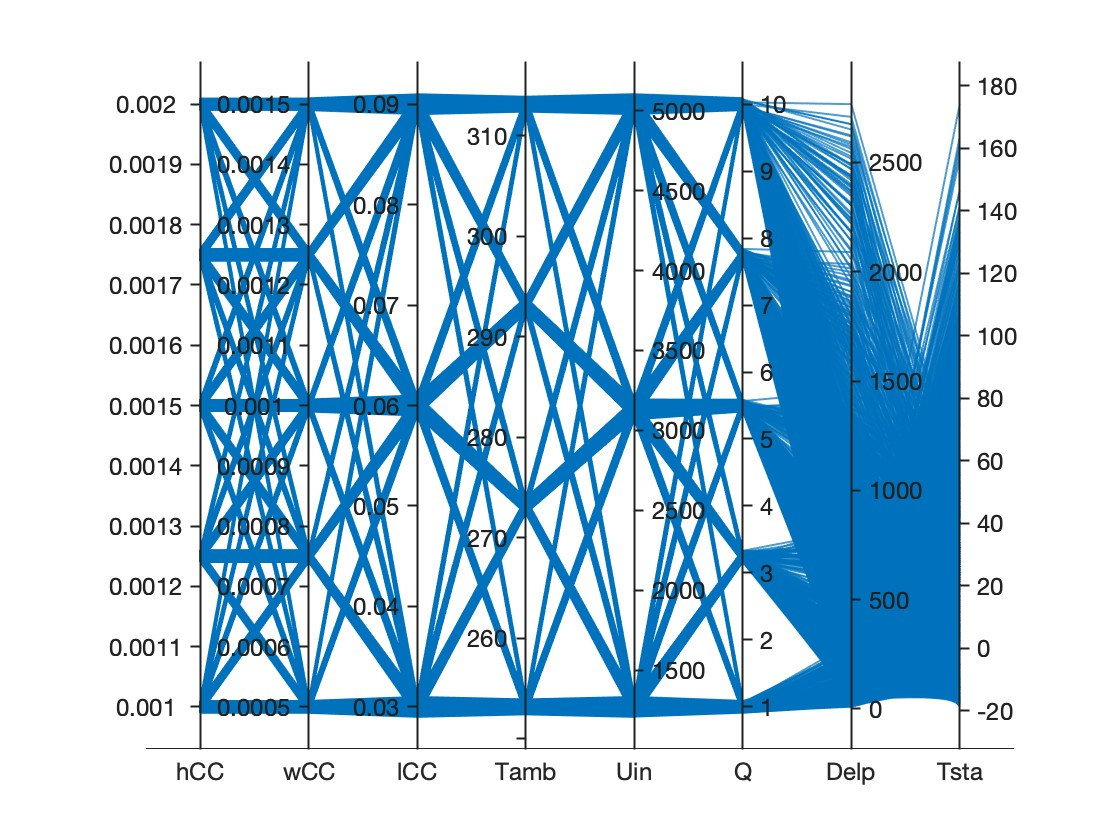
\includegraphics[width=1\textwidth]{00_Images/00_Small_Stack_Images/00_Parallel_Coordinate_Plot_July_10_2024_v1.jpg}  % Change "example-image" to the filename of your image
            \caption{This is an example image.}
            \label{fig:example1}
        \end{figure}

        \begin{figure}[H]
            \centering
            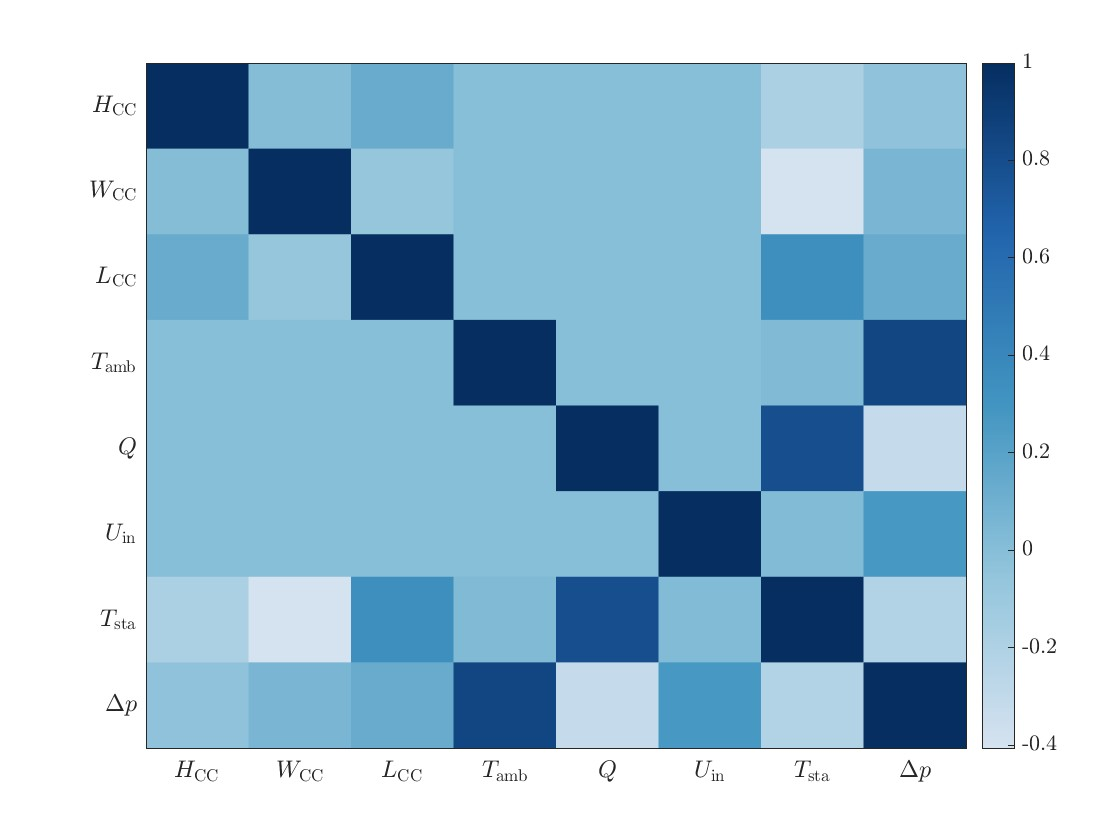
\includegraphics[width=1\textwidth]{00_Images/00_Small_Stack_Images/00_Spearman_Correlation_Matrix_Heatmap_July_10_2024_v1.jpg}  % Change "example-image" to the filename of your image
            \caption{This is an example image.}
            \label{fig:example1}
        \end{figure}

    \subsection{Large Stack}
        \begin{figure}[H]
            \centering
            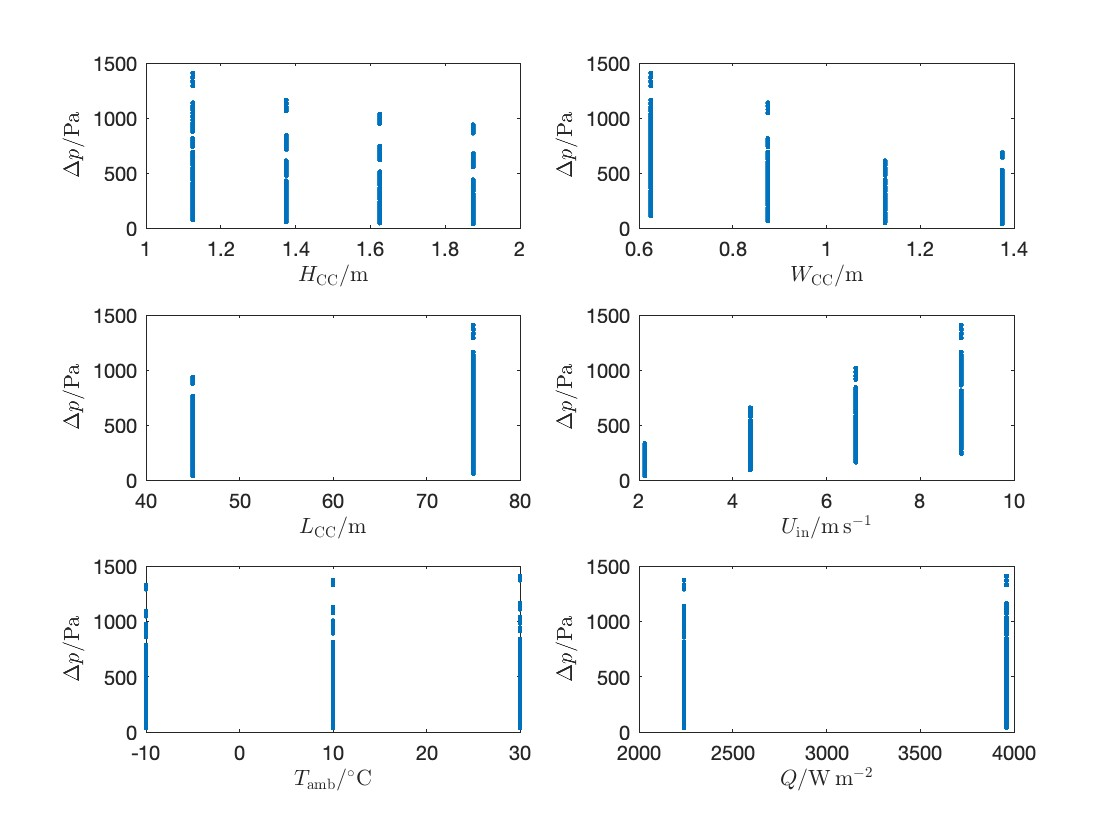
\includegraphics[width=1\textwidth]{00_Images/00_Large_Stack_Images/00_Pressure_Drop_vs_Features_July_10_2024_v1.jpg}  % Change "example-image" to the filename of your image
            \caption{This is an example image.}
            \label{fig:example1}
        \end{figure}

        \begin{figure}[H]
            \centering
            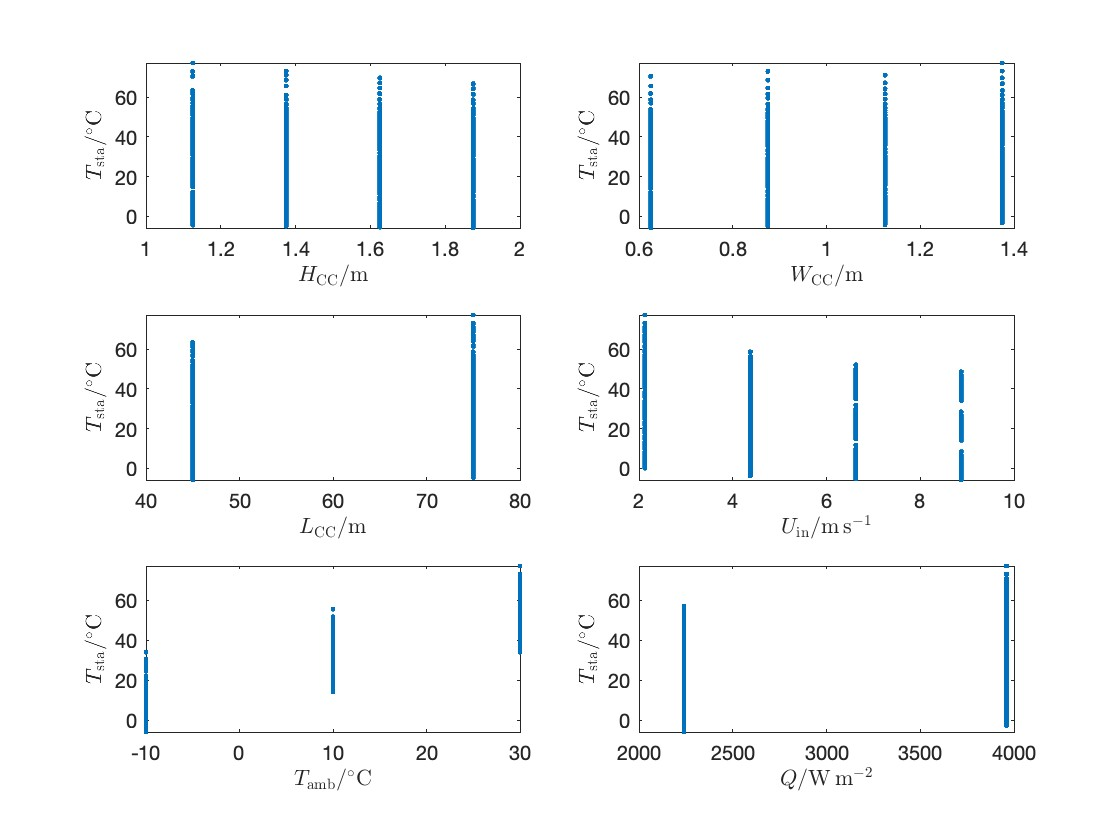
\includegraphics[width=1\textwidth]{00_Images/00_Large_Stack_Images/00_Temperature_vs_Features_July_10_2024_v1.jpg}  % Change "example-image" to the filename of your image
            \caption{This is an example image.}
            \label{fig:example1}
        \end{figure}

        \begin{figure}[H]
            \centering
            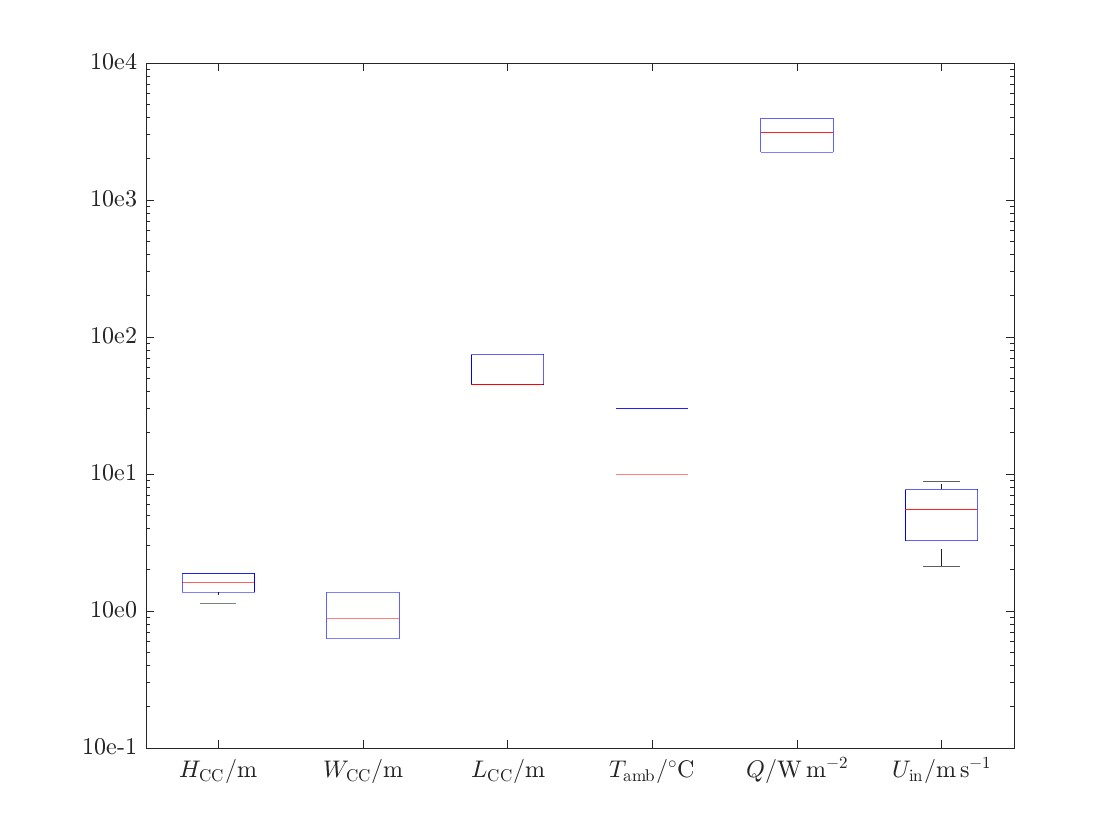
\includegraphics[width=1\textwidth]{00_Images/00_Large_Stack_Images/00_Combined_Boxplot_Features_July_10_2024_v1.jpg}  % Change "example-image" to the filename of your image
            \caption{This is an example image.}
            \label{fig:example1}
        \end{figure}

        \begin{figure}[H]
            \centering
            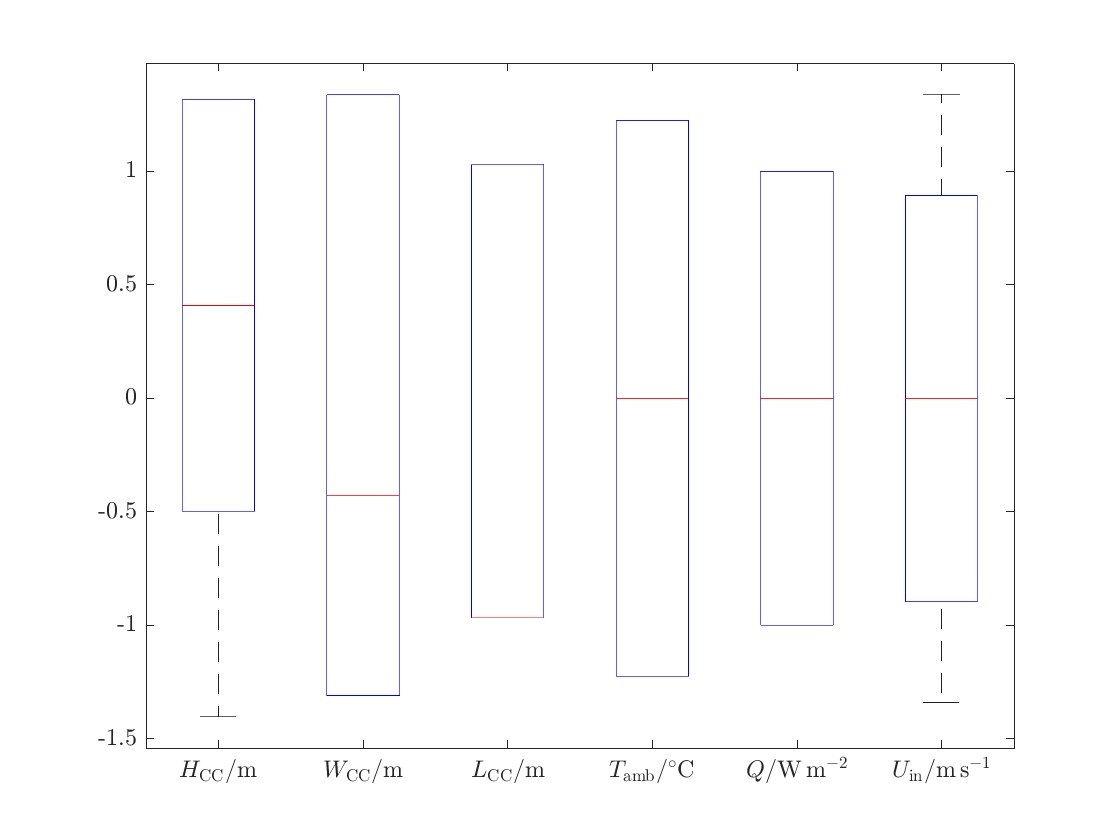
\includegraphics[width=1\textwidth]{00_Images/00_Large_Stack_Images/00_Combined_Boxplot_Normalized_Features_July_10_2024_v1.jpg}  % Change "example-image" to the filename of your image
            \caption{This is an example image.}
            \label{fig:example1}
        \end{figure}

        \begin{figure}[H]
            \centering
            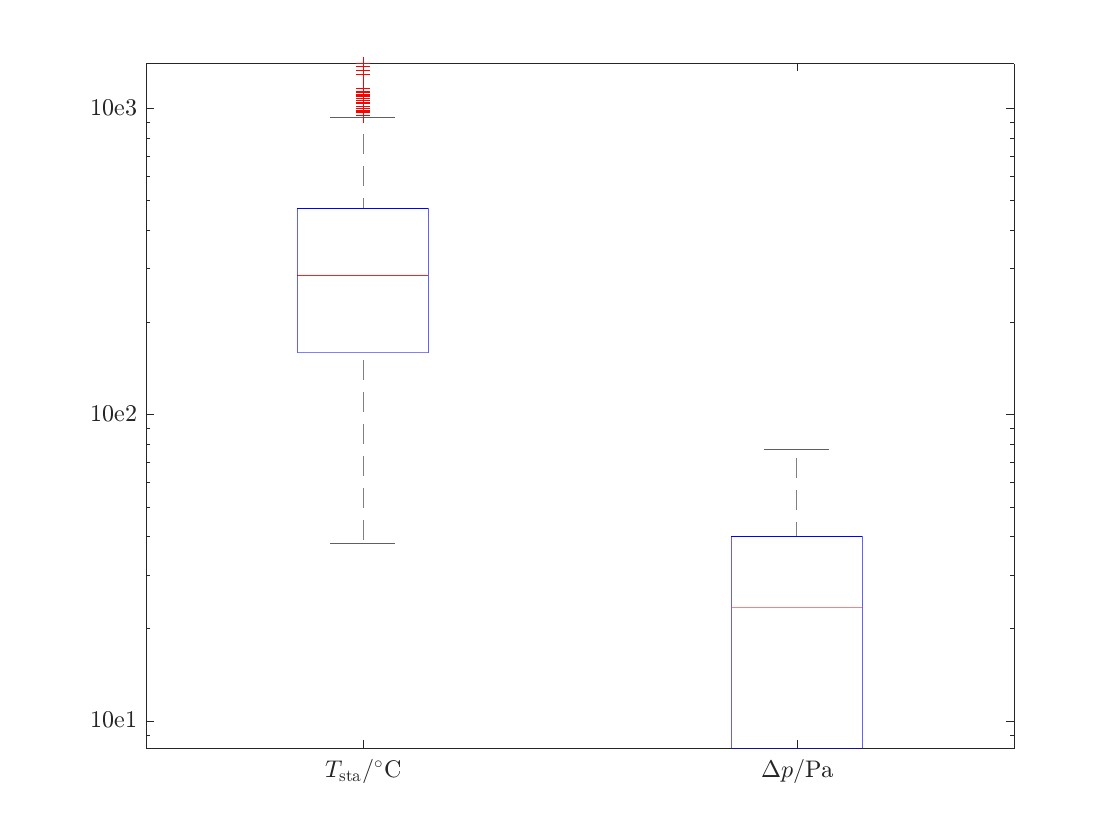
\includegraphics[width=1\textwidth]{00_Images/00_Large_Stack_Images/00_Combined_Boxplot_Outputs_July_10_2024_v1.jpg}  % Change "example-image" to the filename of your image
            \caption{This is an example image.}
            \label{fig:example1}
        \end{figure}

        \begin{figure}[H]
            \centering
            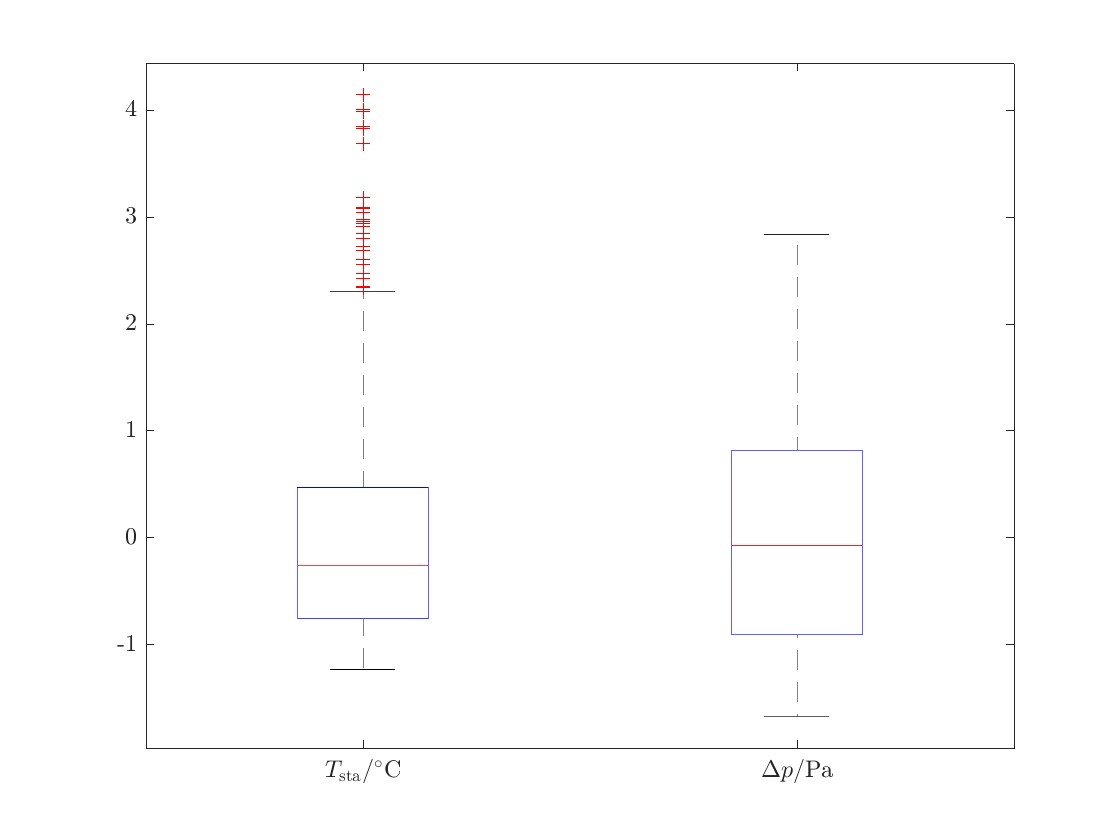
\includegraphics[width=1\textwidth]{00_Images/00_Large_Stack_Images/00_Combined_Boxplot_Normalized_Outputs_July_10_2024_v1.jpg}  % Change "example-image" to the filename of your image
            \caption{This is an example image.}
            \label{fig:example1}
        \end{figure}

        \begin{figure}[H]
            \centering
            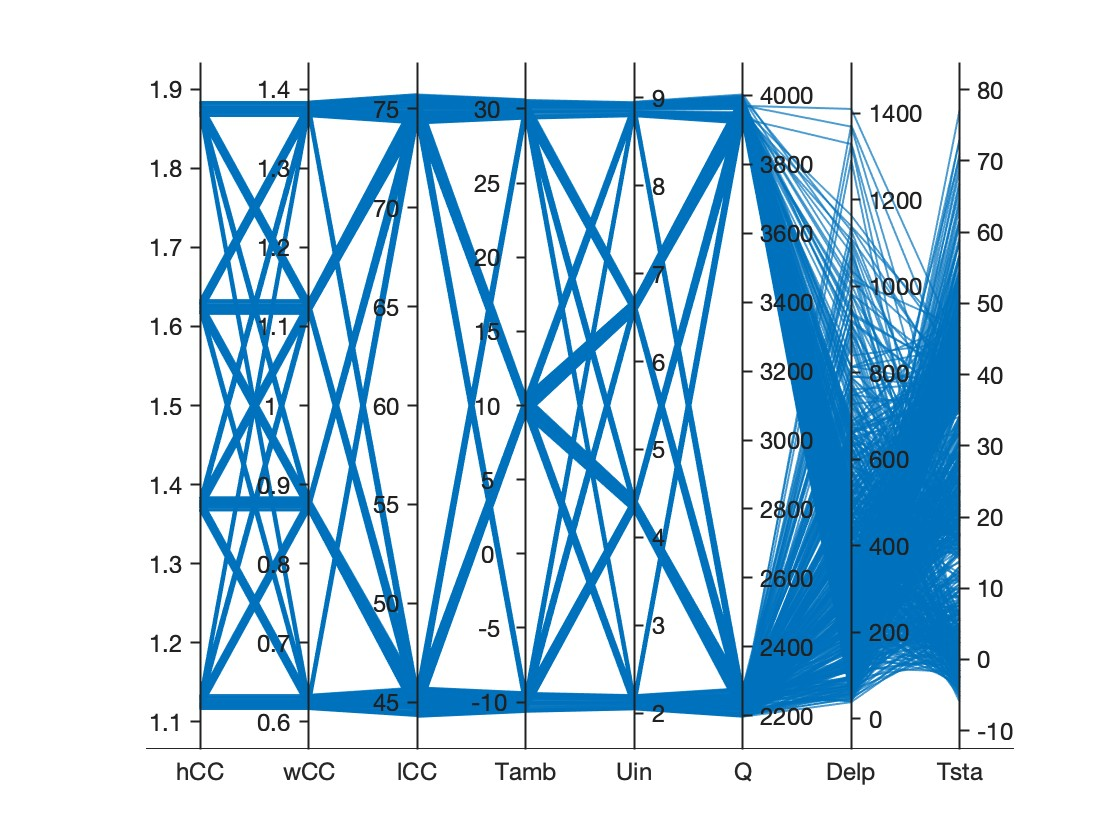
\includegraphics[width=1\textwidth]{00_Images/00_Large_Stack_Images/00_Parallel_Coordinate_Plot_July_10_2024_v1.jpg}  % Change "example-image" to the filename of your image
            \caption{This is an example image.}
            \label{fig:example1}
        \end{figure}

        \begin{figure}[H]
            \centering
            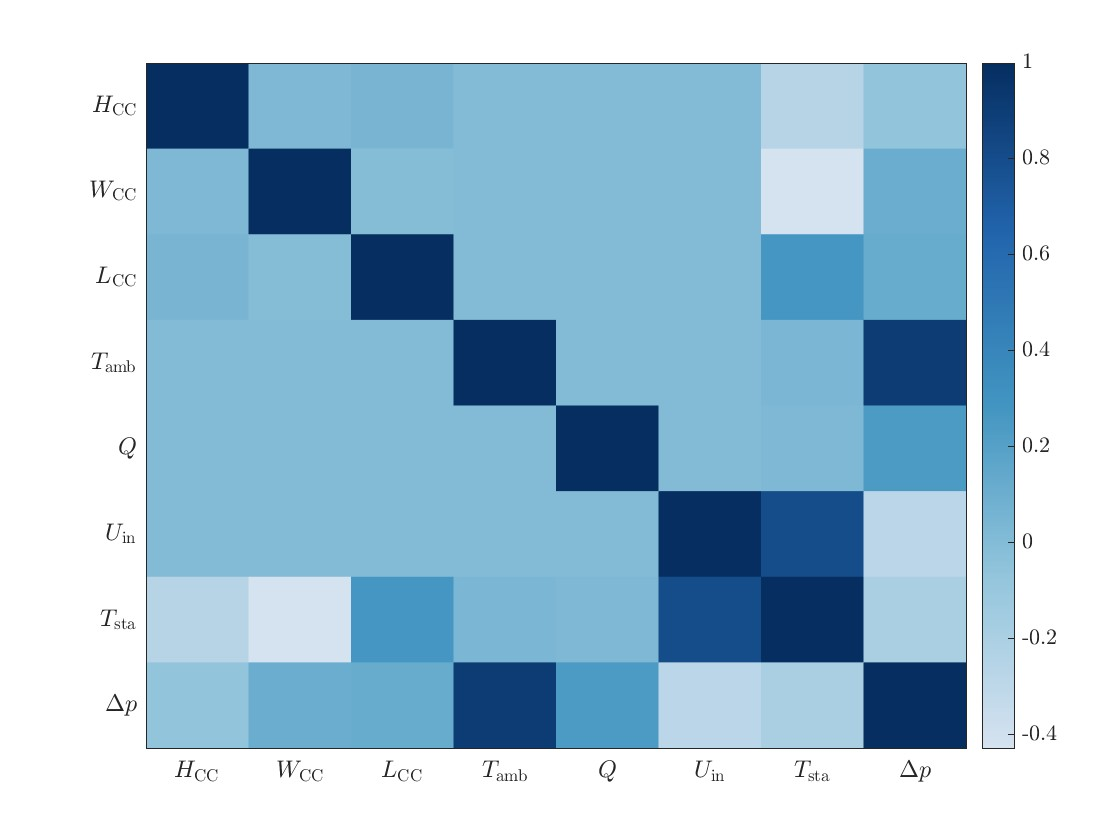
\includegraphics[width=1\textwidth]{00_Images/00_Large_Stack_Images/00_Spearman_Correlation_Matrix_Heatmap_July_10_2024_v1.jpg}  % Change "example-image" to the filename of your image
            \caption{This is an example image.}
            \label{fig:example1}
        \end{figure}

            

\chapter{Training and investigation of different models}

\chapter{Pareto Optimization}

\chapter{Conclusion}

\chapter{Outlook}

\section{References}

\end{document}
